\documentclass[10pt,twocolumn,letterpaper]{article}
\usepackage[review]{cvpr}      % REVIEW version; use [final] for camera-ready
%% This file contains a number of tweaks that are typically applied to the main document.
%% They are not enabled by default, but can be enabled by uncommenting the relevant lines.


%%
%% Official support for 2-column teaser figure
%%
\usepackage{cuted} %< for strip environment

%%
%% For auto-referencing of figures (see fig/teaser.tex and \label{} therein) 
%%
\usepackage{currfile} %< for \currfilebase macro

%%
%% caption and (global) spacing overrides
%%
\usepackage{caption} %< for "\captionof" commands (teaser)
% \setlength{\abovecaptionskip}{.5em} % space above caption
% \setlength{\belowcaptionskip}{1em} % space below caption

%%
%% Inline annotations; for predefined colors, refer to "dvipsnames" in the xcolor package:
%% https://tinyurl.com/overleaf-colors
%%
\newcommand{\red}[1]{{\color{red}#1}}
\newcommand{\todo}[1]{{\color{red}#1}}
\newcommand{\TODO}[1]{\textbf{\color{red}[TODO: #1]}}
%%
%% Disable for camera ready / submission by uncommenting these lines:
%%
% \renewcommand{\TODO}[1]{}
% \renewcommand{\todo}[1]{#1}

%%
%% Work harder in optimizing text layout. Typically shrinks text by 1/6 of page, enable
%% it at the very end of the writing process, when you are just above the page limit.
%%
% \usepackage{microtype}

%%
%% Fine-tune paragraph spacing.
%%
% \renewcommand{\paragraph}[1]{\vspace{.5em}\noindent\textbf{#1.}}

%%
%% Globally adjusts space between figure and caption.
%%
% \setlength{\abovecaptionskip}{.5em}

%%
%% Allows "the use of \paper to refer to the project name"
%% with automatic management of space at the end of the word.
%%
% \usepackage{xspace}
% \newcommand{\paper}{ProjectName\xspace}

%%
%% Commonly used math definitions.
%%
% \DeclareMathOperator*{\argmin}{arg\,min}
% \DeclareMathOperator*{\argmax}{arg\,max}

%%
%% Tighten underline.
%%
% \usepackage{soul}
% \setuldepth{foobar}

%%
%% Reconfigure paragraph (tweaks spacing)
%%

% generated by scripts/paper_numbers.py -- do not edit
\newcommand{\SupRawAcc}{16.5}
\newcommand{\SupRawF}{9.3}
\newcommand{\SupRawTop}{44}
\newcommand{\SupRawAccSd}{1.7}
\newcommand{\SupRawFSd}{1.4}
\newcommand{\SupRawN}{3}
\newcommand{\SupOwnAcc}{30.9}
\newcommand{\SupOwnF}{26.8}
\newcommand{\SupOwnTop}{20}
\newcommand{\SupOwnAccSd}{0.7}
\newcommand{\SupOwnFSd}{0.9}
\newcommand{\SupOwnN}{3}
\newcommand{\SupAdaAcc}{39.0}
\newcommand{\SupAdaF}{32.4}
\newcommand{\SupAdaTop}{22}
\newcommand{\SupAdaAccSd}{1.5}
\newcommand{\SupAdaFSd}{1.3}
\newcommand{\SupAdaN}{3}
\newcommand{\SupAdaSessAcc}{5.3}
\newcommand{\SupAdaSessF}{3.6}
\newcommand{\SupAdaSessTop}{35}
\newcommand{\SupAdaSessAccSd}{0.2}
\newcommand{\SupAdaSessFSd}{0.1}
\newcommand{\SupAdaSessN}{2}
\newcommand{\SwapRawAcc}{27.7}
\newcommand{\SwapRawF}{26.3}
\newcommand{\SwapRawTop}{17}
\newcommand{\SwapRawAccSd}{2.2}
\newcommand{\SwapRawFSd}{1.4}
\newcommand{\SwapRawN}{3}
\newcommand{\SwapBaseRawAcc}{27.1}
\newcommand{\SwapBaseRawF}{23.3}
\newcommand{\SwapBaseRawTop}{23}
\newcommand{\SwapBaseRawAccSd}{2.2}
\newcommand{\SwapBaseRawFSd}{2.0}
\newcommand{\SwapBaseRawN}{3}
\newcommand{\NmRawAcc}{22.9}
\newcommand{\NmRawF}{19.5}
\newcommand{\NmRawTop}{46}
\newcommand{\NmSwapRawAcc}{28.2}
\newcommand{\NmSwapRawF}{23.8}
\newcommand{\NmSwapRawTop}{38}
\newcommand{\NmSwapOwnAcc}{32.7}
\newcommand{\NmSwapOwnF}{28.4}
\newcommand{\NmSwapOwnTop}{14}
\newcommand{\TactSpaceRawAcc}{9.4}
\newcommand{\TactSpaceRawF}{5.3}
\newcommand{\TactSpaceRawTop}{50}
\newcommand{\TactSpaceRawAccSd}{1.0}
\newcommand{\TactSpaceRawFSd}{0.7}
\newcommand{\TactSpaceRawN}{2}
\newcommand{\SupAugRawAcc}{23.6}
\newcommand{\SupAugRawF}{18.6}
\newcommand{\SupAugRawTop}{39}
\newcommand{\SupAugOwnAcc}{37.7}
\newcommand{\SupAugOwnF}{34.0}
\newcommand{\SupAugOwnTop}{18}
\newcommand{\SupSwapRawAcc}{18.8}
\newcommand{\SupSwapRawF}{13.1}
\newcommand{\SupSwapRawTop}{47}
\newcommand{\SupSwapAdaAcc}{43.4}
\newcommand{\SupSwapAdaF}{36.0}
\newcommand{\SupSwapAdaTop}{15}
\newcommand{\SupPrevAcc}{35.8}
\newcommand{\SupPrevF}{31.3}
\newcommand{\SupOnlineAcc}{33.0}
\newcommand{\SupOnlineF}{28.0}
\newcommand{\SupCausalAcc}{30.7}
\newcommand{\SupCausalF}{26.4}
\newcommand{\SupSwapPrevAcc}{39.9}
\newcommand{\SupSwapPrevF}{34.9}
\newcommand{\SupSwapOnlineAcc}{36.3}
\newcommand{\SupSwapOnlineF}{33.0}
\newcommand{\SupSwapCausalAcc}{33.0}
\newcommand{\SupSwapCausalF}{31.1}
\newcommand{\SwapBasePrevAcc}{27.0}
\newcommand{\SwapBasePrevF}{24.2}
\newcommand{\SwapBaseOnlineAcc}{26.3}
\newcommand{\SwapBaseOnlineF}{23.7}
\newcommand{\SwapBaseCausalAcc}{25.4}
\newcommand{\SwapBaseCausalF}{23.1}
\newcommand{\IjepaRawAcc}{11.2}
\newcommand{\IjepaRawF}{6.9}
\newcommand{\IjepaOwnAcc}{40.8}
\newcommand{\IjepaOwnF}{37.5}
\newcommand{\IjepaOwnTop}{13}
\newcommand{\IjepaPrevAcc}{35.5}
\newcommand{\IjepaPrevF}{32.2}
\newcommand{\MaeRawAcc}{10.0}
\newcommand{\MaeRawF}{5.0}
\newcommand{\MaeOwnAcc}{38.1}
\newcommand{\MaeOwnF}{35.4}
\newcommand{\MaeOwnTop}{12}
\newcommand{\MaePrevAcc}{31.6}
\newcommand{\MaePrevF}{28.4}
\newcommand{\SdinoRawAcc}{8.9}
\newcommand{\SdinoRawF}{4.7}
\newcommand{\SdinoOwnAcc}{33.4}
\newcommand{\SdinoOwnF}{31.8}
\newcommand{\SdinoOwnTop}{13}
\newcommand{\SdinoPrevAcc}{26.9}
\newcommand{\SdinoPrevF}{25.4}
\newcommand{\DinovRawAcc}{22.0}
\newcommand{\DinovRawF}{18.9}
\newcommand{\DinovOwnAcc}{39.4}
\newcommand{\DinovOwnF}{35.7}
\newcommand{\DinovOwnTop}{13}
\newcommand{\DinovPrevAcc}{28.3}
\newcommand{\DinovPrevF}{24.5}
\newcommand{\IjepaAdAcc}{34.9}
\newcommand{\IjepaAdF}{31.8}
\newcommand{\IjepaAdTop}{19}
\newcommand{\IjepaAdAccSd}{0.6}
\newcommand{\IjepaAdFSd}{0.5}
\newcommand{\IjepaAdN}{3}
\newcommand{\IjepaAdPrevAcc}{36.4}
\newcommand{\IjepaAdPrevF}{33.7}
\newcommand{\IjepaAdPrevTop}{14}
\newcommand{\IjepaAdPrevAccSd}{0.6}
\newcommand{\IjepaAdPrevFSd}{0.8}
\newcommand{\IjepaAdPrevN}{3}
\newcommand{\MaeAdAcc}{32.6}
\newcommand{\MaeAdF}{28.5}
\newcommand{\MaeAdTop}{20}
\newcommand{\SdinoAdAcc}{28.5}
\newcommand{\SdinoAdF}{22.9}
\newcommand{\SdinoAdTop}{22}
\newcommand{\DinovAdAcc}{25.9}
\newcommand{\DinovAdF}{24.9}
\newcommand{\DinovAdTop}{33}
\newcommand{\IjepaAdNoDecoyAcc}{31.9}
\newcommand{\IjepaAdNoDecoyF}{28.2}
\newcommand{\IjepaAdNoDecoyTop}{24}
\newcommand{\SupFoneRawAcc}{17.3}
\newcommand{\SupFoneRawF}{11.1}
\newcommand{\SupFoneRawTop}{43}
\newcommand{\SupFoneOwnAcc}{44.6}
\newcommand{\SupFoneOwnF}{39.7}
\newcommand{\SupFoneOwnTop}{15}
\newcommand{\SwapFoneRawAcc}{27.6}
\newcommand{\SwapFoneRawF}{25.1}
\newcommand{\SwapFoneRawTop}{14}
\newcommand{\SupFtwoRawAcc}{15.2}
\newcommand{\SupFtwoRawF}{8.5}
\newcommand{\SupFtwoRawTop}{41}
\newcommand{\SupFtwoOwnAcc}{41.5}
\newcommand{\SupFtwoOwnF}{37.5}
\newcommand{\SupFtwoOwnTop}{18}
\newcommand{\SwapFtwoRawAcc}{24.7}
\newcommand{\SwapFtwoRawF}{22.0}
\newcommand{\SwapFtwoRawTop}{16}
\newcommand{\SupFfourRawAcc}{14.0}
\newcommand{\SupFfourRawF}{8.1}
\newcommand{\SupFfourRawTop}{44}
\newcommand{\SupFfourOwnAcc}{37.6}
\newcommand{\SupFfourOwnF}{34.4}
\newcommand{\SupFfourOwnTop}{21}
\newcommand{\SwapFfourRawAcc}{24.5}
\newcommand{\SwapFfourRawF}{22.8}
\newcommand{\SwapFfourRawTop}{14}
\newcommand{\SupFonePrevAcc}{50.8}
\newcommand{\SupFonePrevF}{45.9}
\newcommand{\SupFtwoPrevAcc}{43.9}
\newcommand{\SupFtwoPrevF}{39.0}
\newcommand{\SupFfourPrevAcc}{37.8}
\newcommand{\SupFfourPrevF}{32.8}
\newcommand{\SupFoneSeedsPrevAcc}{51.0}
\newcommand{\SupFoneSeedsPrevAccSd}{0.5}
\newcommand{\SupFoneSeedsPrevN}{3}
\newcommand{\SupSwapFonePrevAcc}{52.4}
\newcommand{\SupSwapFonePrevF}{46.5}
\newcommand{\SupAugFonePrevAcc}{54.3}
\newcommand{\SupAugFonePrevF}{48.7}
\newcommand{\SwapFonePrevAcc}{31.0}
\newcommand{\SwapFonePrevF}{27.8}
\newcommand{\SupSwapFoneRawAcc}{28.4}
\newcommand{\SupSwapFoneRawF}{22.1}
\newcommand{\SupSwapFoneRawTop}{31}
\newcommand{\SupAugFoneRawAcc}{45.2}
\newcommand{\SupAugFoneRawF}{41.6}
\newcommand{\SupAugFoneRawTop}{23}
\newcommand{\SupFoneRawSAcc}{16.6}
\newcommand{\SupFoneRawSF}{10.5}
\newcommand{\SupFoneRawSTop}{42}
\newcommand{\SupFoneRawSAccSd}{0.8}
\newcommand{\SupFoneRawSFSd}{1.0}
\newcommand{\SupFoneRawSN}{3}
\newcommand{\SupFonePrevRawHeadAcc}{51.0}
\newcommand{\SupFonePrevRawHeadF}{45.9}
\newcommand{\SupFonePrevRawHeadAccSd}{0.5}
\newcommand{\SupFonePrevRawHeadN}{3}
\newcommand{\SupAugFoneRawSAcc}{43.9}
\newcommand{\SupAugFoneRawSF}{40.3}
\newcommand{\SupAugFoneRawSTop}{24}
\newcommand{\SupAugFoneRawSAccSd}{2.3}
\newcommand{\SupAugFoneRawSFSd}{2.5}
\newcommand{\SupAugFoneRawSN}{3}
\newcommand{\SupAugFonePrevRawHeadAcc}{54.0}
\newcommand{\SupAugFonePrevRawHeadF}{48.3}
\newcommand{\SupAugFonePrevRawHeadAccSd}{0.9}
\newcommand{\SupAugFonePrevRawHeadN}{3}
\newcommand{\SwapFoneRawSAcc}{26.5}
\newcommand{\SwapFoneRawSF}{23.6}
\newcommand{\SwapFoneRawSTop}{16}
\newcommand{\SwapFoneRawSAccSd}{1.6}
\newcommand{\SwapFoneRawSFSd}{1.9}
\newcommand{\SwapFoneRawSN}{3}
\newcommand{\SupAugSwapFoneRawAcc}{44.1}
\newcommand{\SupAugSwapFoneRawF}{39.2}
\newcommand{\SupAugSwapFoneRawTop}{26}
\newcommand{\SupAugSwapFonePrevSAcc}{54.6}
\newcommand{\SupAugSwapFonePrevSF}{48.0}
\newcommand{\SupAugSwapFonePrevSAccSd}{0.0}
\newcommand{\SupAugSwapFonePrevSN}{1}
\newcommand{\SupSwapFonePrevSAcc}{52.4}
\newcommand{\SupSwapFonePrevSF}{46.5}
\newcommand{\SupSwapFonePrevSAccSd}{0.0}
\newcommand{\SupSwapFonePrevSN}{1}
\newcommand{\SupAugRawSAcc}{22.7}
\newcommand{\SupAugRawSF}{17.7}
\newcommand{\SupAugRawSTop}{36}
\newcommand{\SupAugRawSAccSd}{1.2}
\newcommand{\SupAugRawSFSd}{1.3}
\newcommand{\SupAugRawSN}{2}
\newcommand{\SupFoneScHalfRawAcc}{21.5}
\newcommand{\SupFoneScHalfRawF}{15.4}
\newcommand{\SupFoneScHalfRawTop}{39}
\newcommand{\SupFoneScHalfPrevSAcc}{52.9}
\newcommand{\SupFoneScHalfPrevSF}{48.5}
\newcommand{\SupFoneScHalfPrevSAccSd}{0.0}
\newcommand{\SupFoneScHalfPrevSN}{1}
\newcommand{\SupFoneScQuarterRawAcc}{23.1}
\newcommand{\SupFoneScQuarterRawF}{17.1}
\newcommand{\SupFoneScQuarterRawTop}{41}
\newcommand{\SupFoneScQuarterPrevSAcc}{49.6}
\newcommand{\SupFoneScQuarterPrevSF}{43.5}
\newcommand{\SupFoneScQuarterPrevSAccSd}{0.0}
\newcommand{\SupFoneScQuarterPrevSN}{1}
\newcommand{\SupScHalfOwnAcc}{30.9}
\newcommand{\SupScHalfOwnF}{27.1}
\newcommand{\SupScHalfOwnTop}{21}
\newcommand{\SwapScHalfRawAcc}{27.6}
\newcommand{\SwapScHalfRawF}{25.5}
\newcommand{\SwapScHalfRawTop}{17}
\newcommand{\SupScQuarterOwnAcc}{28.6}
\newcommand{\SupScQuarterOwnF}{24.9}
\newcommand{\SupScQuarterOwnTop}{25}
\newcommand{\SwapScQuarterRawAcc}{25.4}
\newcommand{\SwapScQuarterRawF}{22.8}
\newcommand{\SwapScQuarterRawTop}{18}
\newcommand{\GapSupBRawAcc}{45.3}
\newcommand{\GapSupBRawF}{38.6}
\newcommand{\GapSupBRawTop}{17}
\newcommand{\GapSupDRawAcc}{23.5}
\newcommand{\GapSupDRawF}{16.9}
\newcommand{\GapSupDRawTop}{32}
\newcommand{\GapSupBOwnAcc}{59.3}
\newcommand{\GapSupBOwnF}{56.5}
\newcommand{\GapSupBOwnTop}{13}
\newcommand{\GapSupDOwnAcc}{35.2}
\newcommand{\GapSupDOwnF}{26.9}
\newcommand{\GapSupDOwnTop}{15}
\newcommand{\GapSwapBRawAcc}{46.6}
\newcommand{\GapSwapBRawF}{46.5}
\newcommand{\GapSwapBRawTop}{10}
\newcommand{\GapSwapDRawAcc}{24.3}
\newcommand{\GapSwapDRawF}{19.4}
\newcommand{\GapSwapDRawTop}{21}
\newcommand{\GapSwapBOwnAcc}{39.0}
\newcommand{\GapSwapBOwnF}{38.5}
\newcommand{\GapSwapBOwnTop}{16}
\newcommand{\GapSwapDOwnAcc}{23.7}
\newcommand{\GapSwapDOwnF}{19.6}
\newcommand{\GapSwapDOwnTop}{14}
\newcommand{\GapIjepaAdBRawAcc}{49.2}
\newcommand{\GapIjepaAdBRawF}{46.5}
\newcommand{\GapIjepaAdBRawTop}{13}
\newcommand{\GapIjepaAdDRawAcc}{31.0}
\newcommand{\GapIjepaAdDRawF}{24.9}
\newcommand{\GapIjepaAdDRawTop}{17}
\newcommand{\ForceGeomFreshR}{0.43}
\newcommand{\ForceGeomFreshC}{0.66}
\newcommand{\ForceGeomPrevR}{0.48}
\newcommand{\ForceGeomPrevC}{0.71}
\newcommand{\ForceGeomXeraR}{0.48}
\newcommand{\ForceGeomXeraC}{0.72}
\newcommand{\ForceWithinRho}{0.70}
\newcommand{\ForceLearnedBestR}{0.11}
\newcommand{\ContactRefRecall}{99.9}
\newcommand{\ContactRefSpec}{86.2}
\newcommand{\ContactRawSpec}{0}
\newcommand{\ContactBlankdiffSpec}{72.2}
\newcommand{\ContactBlankdiffSpecMin}{72}
\newcommand{\ContactBlankdiffSpecMax}{89}
\newcommand{\SigOwn}{0.53}
\newcommand{\SigSameDay}{0.41}
\newcommand{\SigOtherEra}{0.15}
\newcommand{\SigOtherGel}{0.16}
\newcommand{\SigCOwn}{0.53}
\newcommand{\SigCSameDay}{0.41}
\newcommand{\SigSameEraOtherDay}{0.38}
\newcommand{\SigCOtherEra}{0.18}
\newcommand{\SigCOtherGel}{0.16}
\newcommand{\TmSigOwn}{0.41}
\newcommand{\TmSigSameDay}{0.39}
\newcommand{\TmSigOtherDay}{0.34}
\newcommand{\TmSigOtherGel}{0.19}
\newcommand{\RerenderRealA}{5.9}
\newcommand{\RerenderRealB}{52.4}
\newcommand{\RerenderAtoB}{35.3}
\newcommand{\RerenderAtoA}{7.5}
\newcommand{\TmLaterSupRawAcc}{19.6}
\newcommand{\TmLaterSupRawF}{11.8}
\newcommand{\TmLaterSupRawTop}{47}
\newcommand{\TmLaterSupPrevAcc}{19.9}
\newcommand{\TmLaterSupPrevF}{18.0}
\newcommand{\TmLaterSupPrevTop}{23}
\newcommand{\TmLaterSupAdaRunAcc}{24.1}
\newcommand{\TmLaterSupAdaRunF}{21.1}
\newcommand{\TmLaterSupAdaRunTop}{23}
\newcommand{\TmLaterSupOwnAcc}{17.6}
\newcommand{\TmLaterSupOwnF}{14.8}
\newcommand{\TmLaterSupOwnTop}{29}
\newcommand{\TmLaterIjepaRawAcc}{10.0}
\newcommand{\TmLaterIjepaRawF}{4.2}
\newcommand{\TmLaterIjepaRawTop}{84}
\newcommand{\TmLaterIjepaPrevAcc}{17.5}
\newcommand{\TmLaterIjepaPrevF}{16.5}
\newcommand{\TmLaterIjepaPrevTop}{26}
\newcommand{\TmLaterSwapRawAcc}{17.4}
\newcommand{\TmLaterSwapRawF}{13.2}
\newcommand{\TmLaterSwapRawTop}{47}
\newcommand{\TmLaterSwapPrevAcc}{19.8}
\newcommand{\TmLaterSwapPrevF}{19.1}
\newcommand{\TmLaterSwapPrevTop}{21}
\newcommand{\TmLaterSwapAdaRunAcc}{25.1}
\newcommand{\TmLaterSwapAdaRunF}{21.4}
\newcommand{\TmLaterSwapAdaRunTop}{27}
\newcommand{\TmLaterSwapOwnAcc}{21.6}
\newcommand{\TmLaterSwapOwnF}{20.8}
\newcommand{\TmLaterSwapOwnTop}{26}
\newcommand{\TmLaterIjepaAdRawAcc}{16.7}
\newcommand{\TmLaterIjepaAdRawF}{11.1}
\newcommand{\TmLaterIjepaAdRawTop}{85}
\newcommand{\TmLaterIjepaAdPrevAcc}{14.3}
\newcommand{\TmLaterIjepaAdPrevF}{13.8}
\newcommand{\TmLaterIjepaAdPrevTop}{34}
\newcommand{\TmGelSupRawAcc}{24.2}
\newcommand{\TmGelSupRawF}{20.8}
\newcommand{\TmGelSupRawTop}{37}
\newcommand{\TmGelSupPrevAcc}{27.3}
\newcommand{\TmGelSupPrevF}{25.5}
\newcommand{\TmGelSupPrevTop}{20}
\newcommand{\TmGelSupAdaRunAcc}{32.0}
\newcommand{\TmGelSupAdaRunF}{30.8}
\newcommand{\TmGelSupAdaRunTop}{25}
\newcommand{\TmGelSupOwnAcc}{28.3}
\newcommand{\TmGelSupOwnF}{26.9}
\newcommand{\TmGelSupOwnTop}{24}
\newcommand{\TmGelIjepaRawAcc}{13.2}
\newcommand{\TmGelIjepaRawF}{8.0}
\newcommand{\TmGelIjepaRawTop}{52}
\newcommand{\TmGelIjepaPrevAcc}{19.8}
\newcommand{\TmGelIjepaPrevF}{18.4}
\newcommand{\TmGelIjepaPrevTop}{25}
\newcommand{\TmGelSwapRawAcc}{13.4}
\newcommand{\TmGelSwapRawF}{9.9}
\newcommand{\TmGelSwapRawTop}{58}
\newcommand{\TmGelSwapPrevAcc}{20.2}
\newcommand{\TmGelSwapPrevF}{18.7}
\newcommand{\TmGelSwapPrevTop}{27}
\newcommand{\TmGelSwapAdaRunAcc}{17.2}
\newcommand{\TmGelSwapAdaRunF}{13.2}
\newcommand{\TmGelSwapAdaRunTop}{35}
\newcommand{\TmGelSwapOwnAcc}{23.2}
\newcommand{\TmGelSwapOwnF}{22.5}
\newcommand{\TmGelSwapOwnTop}{22}
\newcommand{\TmGelIjepaAdRawAcc}{13.9}
\newcommand{\TmGelIjepaAdRawF}{9.8}
\newcommand{\TmGelIjepaAdRawTop}{42}
\newcommand{\TmGelIjepaAdPrevAcc}{18.2}
\newcommand{\TmGelIjepaAdPrevF}{16.6}
\newcommand{\TmGelIjepaAdPrevTop}{34}
\newcommand{\SupFoneRawEighteen}{19.2}
\newcommand{\SupAugFoneRawEighteen}{46.1}
\newcommand{\IjepaAdEighteen}{35.1}
\newcommand{\IjepaRawEighteen}{12.5}
\newcommand{\SupFoneRawFSOne}{36.8}
\newcommand{\SupFoneRawFSFive}{58.8}
\newcommand{\SupFoneRawFSTen}{70.1}
\newcommand{\SupFoneOwnFSOne}{51.4}
\newcommand{\SupFoneOwnFSFive}{63.2}
\newcommand{\SupFoneOwnFSTen}{73.4}
\newcommand{\SupAugFoneRawFSOne}{49.0}
\newcommand{\SupAugFoneRawFSFive}{62.5}
\newcommand{\SupAugFoneRawFSTen}{69.8}
\newcommand{\SupAugFoneOwnFSOne}{53.5}
\newcommand{\SupAugFoneOwnFSFive}{65.3}
\newcommand{\SupAugFoneOwnFSTen}{72.2}
\newcommand{\IjepaAdFSOne}{39.7}
\newcommand{\IjepaAdFSFive}{46.2}
\newcommand{\IjepaAdFSTen}{52.2}
\newcommand{\SupFoneAdaAcc}{49.1}
\newcommand{\SupFoneAdaF}{45.7}
\newcommand{\SupFoneAdaTop}{16}
\newcommand{\SupFoneAdaSessAcc}{6.2}
\newcommand{\SupFoneAdaSessF}{3.6}
\newcommand{\SupFoneAdaSessTop}{32}
\newcommand{\SupAugFoneAdaAcc}{40.4}
\newcommand{\SupAugFoneAdaF}{38.3}
\newcommand{\SupAugFoneAdaTop}{19}
\newcommand{\SupFonePrevSAcc}{50.5}
\newcommand{\SupFonePrevSF}{45.6}
\newcommand{\SupFonePrevSTop}{11}
\newcommand{\SupFonePrevSAccSd}{0.7}
\newcommand{\SupFonePrevSN}{3}
\newcommand{\SupAugFonePrevSAcc}{53.8}
\newcommand{\SupAugFonePrevSF}{49.3}
\newcommand{\SupAugFonePrevSTop}{13}
\newcommand{\SupAugFonePrevSAccSd}{1.6}
\newcommand{\SupAugFonePrevSN}{3}
\newcommand{\SupFoneOnlineSAcc}{46.6}
\newcommand{\SupFoneOnlineSF}{41.1}
\newcommand{\SupFoneOnlineSTop}{16}
\newcommand{\SupFoneOnlineSAccSd}{0.8}
\newcommand{\SupFoneOnlineSN}{3}
\newcommand{\SupAugFoneOnlineSAcc}{49.6}
\newcommand{\SupAugFoneOnlineSF}{44.0}
\newcommand{\SupAugFoneOnlineSTop}{16}
\newcommand{\SupAugFoneOnlineSAccSd}{1.6}
\newcommand{\SupAugFoneOnlineSN}{3}
\newcommand{\SupFoneOwnSAcc}{47.7}
\newcommand{\SupFoneOwnSF}{41.6}
\newcommand{\SupFoneOwnSTop}{15}
\newcommand{\SupFoneOwnSAccSd}{0.9}
\newcommand{\SupFoneOwnSN}{3}
\newcommand{\DannFoneRawAcc}{18.3}
\newcommand{\DannFoneRawF}{11.7}
\newcommand{\DannFoneRawTop}{43}
\newcommand{\DannFoneAdaAcc}{47.9}
\newcommand{\DannFoneAdaF}{45.2}
\newcommand{\DannFoneAdaTop}{16}
\newcommand{\DannFonePrevAcc}{52.9}
\newcommand{\DannFonePrevF}{48.0}
\newcommand{\DannFonePrevTop}{12}
\newcommand{\DannFonePrevAccSd}{0.0}
\newcommand{\DannFonePrevN}{1}
\newcommand{\NoiseFeightRawAcc}{14.7}
\newcommand{\NoiseFeightRawF}{8.4}
\newcommand{\NoiseFeightRawTop}{46}
\newcommand{\NoiseFeightPrevAcc}{34.0}
\newcommand{\NoiseFeightPrevF}{30.7}
\newcommand{\NoiseFeightPrevTop}{18}
\newcommand{\NoiseFeightPrevAccSd}{0.0}
\newcommand{\NoiseFeightPrevN}{1}
\newcommand{\NoiseAugFeightRawAcc}{26.6}
\newcommand{\NoiseAugFeightRawF}{23.2}
\newcommand{\NoiseAugFeightRawTop}{31}
\newcommand{\NoiseAugFeightPrevAcc}{38.7}
\newcommand{\NoiseAugFeightPrevF}{34.9}
\newcommand{\NoiseAugFeightPrevTop}{17}
\newcommand{\NoiseAugFeightPrevAccSd}{0.0}
\newcommand{\NoiseAugFeightPrevN}{1}
\newcommand{\SupAugPrevAcc}{40.7}
\newcommand{\SupAugPrevF}{35.9}
\newcommand{\SupFonePrevFSOne}{55.5}
\newcommand{\SupFonePrevFSFive}{68.9}
\newcommand{\SupFonePrevFSTen}{76.5}
\newcommand{\SupFoneTrainCalFSOne}{42.6}
\newcommand{\SupFoneTrainCalFSFive}{62.7}
\newcommand{\SupFoneTrainCalFSTen}{75.0}
\newcommand{\SupAugFonePrevFSOne}{56.3}
\newcommand{\SupAugFonePrevFSFive}{68.3}
\newcommand{\SupAugFonePrevFSTen}{73.5}
\newcommand{\SupAugFoneTrainCalFSOne}{49.7}
\newcommand{\SupAugFoneTrainCalFSFive}{60.6}
\newcommand{\SupAugFoneTrainCalFSTen}{67.9}
\newcommand{\HoldSupRawAcc}{54.4}
\newcommand{\HoldSupRawF}{55.7}
\newcommand{\HoldSupRawTop}{16}
\newcommand{\HoldSupOwnAcc}{54.8}
\newcommand{\HoldSupOwnF}{53.9}
\newcommand{\HoldSupOwnTop}{22}
\newcommand{\HoldSupAdaAcc}{47.5}
\newcommand{\HoldSupAdaF}{48.1}
\newcommand{\HoldSupAdaTop}{18}
\newcommand{\HoldSupAdaSessAcc}{2.6}
\newcommand{\HoldSupAdaSessF}{2.9}
\newcommand{\HoldSupAdaSessTop}{48}
\newcommand{\HoldSupPrevAcc}{59.2}
\newcommand{\HoldSupPrevF}{61.5}
\newcommand{\HoldSupPrevTop}{11}
\newcommand{\HoldSupPrevAccSd}{0.0}
\newcommand{\HoldSupPrevN}{1}
\newcommand{\HoldSupOnlineAcc}{51.9}
\newcommand{\HoldSupOnlineF}{53.1}
\newcommand{\HoldSupOnlineTop}{12}
\newcommand{\HoldSupOnlineAccSd}{0.0}
\newcommand{\HoldSupOnlineN}{1}
\newcommand{\HoldAugRawAcc}{57.9}
\newcommand{\HoldAugRawF}{57.7}
\newcommand{\HoldAugRawTop}{20}
\newcommand{\HoldAugOwnAcc}{55.2}
\newcommand{\HoldAugOwnF}{55.0}
\newcommand{\HoldAugOwnTop}{20}
\newcommand{\HoldAugAdaAcc}{42.2}
\newcommand{\HoldAugAdaF}{43.6}
\newcommand{\HoldAugAdaTop}{23}
\newcommand{\HoldAugAdaSessAcc}{3.4}
\newcommand{\HoldAugAdaSessF}{1.9}
\newcommand{\HoldAugAdaSessTop}{39}
\newcommand{\HoldAugPrevAcc}{61.3}
\newcommand{\HoldAugPrevF}{61.5}
\newcommand{\HoldAugPrevTop}{19}
\newcommand{\HoldAugPrevAccSd}{0.0}
\newcommand{\HoldAugPrevN}{1}
\newcommand{\HoldAugOnlineAcc}{58.1}
\newcommand{\HoldAugOnlineF}{59.1}
\newcommand{\HoldAugOnlineTop}{21}
\newcommand{\HoldAugOnlineAccSd}{0.0}
\newcommand{\HoldAugOnlineN}{1}
\newcommand{\HoldSwapRawAcc}{27.0}
\newcommand{\HoldSwapRawF}{31.5}
\newcommand{\HoldSwapRawTop}{20}
\newcommand{\HoldSwapOwnAcc}{25.9}
\newcommand{\HoldSwapOwnF}{31.4}
\newcommand{\HoldSwapOwnTop}{20}
\newcommand{\HoldSwapAdaAcc}{1.6}
\newcommand{\HoldSwapAdaF}{2.5}
\newcommand{\HoldSwapAdaTop}{60}
\newcommand{\HoldSwapAdaSessAcc}{0.0}
\newcommand{\HoldSwapAdaSessF}{0.0}
\newcommand{\HoldSwapAdaSessTop}{70}
\newcommand{\HoldSwapPrevAcc}{20.9}
\newcommand{\HoldSwapPrevF}{26.0}
\newcommand{\HoldSwapPrevTop}{23}
\newcommand{\HoldSwapPrevAccSd}{0.0}
\newcommand{\HoldSwapPrevN}{1}
\newcommand{\HoldSwapOnlineAcc}{22.9}
\newcommand{\HoldSwapOnlineF}{28.1}
\newcommand{\HoldSwapOnlineTop}{21}
\newcommand{\HoldSwapOnlineAccSd}{0.0}
\newcommand{\HoldSwapOnlineN}{1}
\newcommand{\HoldFeightRawAcc}{39.0}
\newcommand{\HoldFeightRawF}{37.6}
\newcommand{\HoldFeightRawTop}{23}
\newcommand{\HoldFeightOwnAcc}{40.5}
\newcommand{\HoldFeightOwnF}{40.6}
\newcommand{\HoldFeightOwnTop}{17}
\newcommand{\HoldFeightAdaAcc}{40.4}
\newcommand{\HoldFeightAdaF}{43.5}
\newcommand{\HoldFeightAdaTop}{26}
\newcommand{\HoldFeightAdaSessAcc}{2.1}
\newcommand{\HoldFeightAdaSessF}{3.0}
\newcommand{\HoldFeightAdaSessTop}{65}
\newcommand{\HoldFeightPrevAcc}{37.9}
\newcommand{\HoldFeightPrevF}{41.8}
\newcommand{\HoldFeightPrevTop}{13}
\newcommand{\HoldFeightPrevAccSd}{0.0}
\newcommand{\HoldFeightPrevN}{1}
\newcommand{\HoldFeightOnlineAcc}{32.4}
\newcommand{\HoldFeightOnlineF}{33.9}
\newcommand{\HoldFeightOnlineTop}{16}
\newcommand{\HoldFeightOnlineAccSd}{0.0}
\newcommand{\HoldFeightOnlineN}{1}
\newcommand{\GapFoneSupBRawAcc}{68.4}
\newcommand{\GapFoneSupBRawF}{67.5}
\newcommand{\GapFoneSupBRawTop}{15}
\newcommand{\GapFoneSupBOwnAcc}{69.9}
\newcommand{\GapFoneSupBOwnF}{68.0}
\newcommand{\GapFoneSupBOwnTop}{13}
\newcommand{\GapFoneSupBAdaAcc}{77.1}
\newcommand{\GapFoneSupBAdaF}{75.2}
\newcommand{\GapFoneSupBAdaTop}{11}
\newcommand{\GapFoneSupBPrevAcc}{80.6}
\newcommand{\GapFoneSupBPrevF}{78.4}
\newcommand{\GapFoneSupBPrevTop}{12}
\newcommand{\GapFoneSupBPrevAccSd}{0.0}
\newcommand{\GapFoneSupBPrevN}{1}
\newcommand{\GapFoneSupDRawAcc}{39.1}
\newcommand{\GapFoneSupDRawF}{29.4}
\newcommand{\GapFoneSupDRawTop}{18}
\newcommand{\GapFoneSupDOwnAcc}{43.5}
\newcommand{\GapFoneSupDOwnF}{35.4}
\newcommand{\GapFoneSupDOwnTop}{16}
\newcommand{\GapFoneSupDAdaAcc}{30.2}
\newcommand{\GapFoneSupDAdaF}{25.7}
\newcommand{\GapFoneSupDAdaTop}{22}
\newcommand{\GapFoneSupDPrevAcc}{37.3}
\newcommand{\GapFoneSupDPrevF}{30.9}
\newcommand{\GapFoneSupDPrevTop}{17}
\newcommand{\GapFoneSupDPrevAccSd}{0.0}
\newcommand{\GapFoneSupDPrevN}{1}
\newcommand{\GapFoneAugBRawAcc}{71.0}
\newcommand{\GapFoneAugBRawF}{69.0}
\newcommand{\GapFoneAugBRawTop}{19}
\newcommand{\GapFoneAugBOwnAcc}{70.4}
\newcommand{\GapFoneAugBOwnF}{68.1}
\newcommand{\GapFoneAugBOwnTop}{19}
\newcommand{\GapFoneAugBAdaAcc}{66.0}
\newcommand{\GapFoneAugBAdaF}{63.4}
\newcommand{\GapFoneAugBAdaTop}{16}
\newcommand{\GapFoneAugBPrevAcc}{73.3}
\newcommand{\GapFoneAugBPrevF}{71.1}
\newcommand{\GapFoneAugBPrevTop}{19}
\newcommand{\GapFoneAugBPrevAccSd}{0.0}
\newcommand{\GapFoneAugBPrevN}{1}
\newcommand{\GapFoneAugDRawAcc}{43.4}
\newcommand{\GapFoneAugDRawF}{36.0}
\newcommand{\GapFoneAugDRawTop}{16}
\newcommand{\GapFoneAugDOwnAcc}{42.4}
\newcommand{\GapFoneAugDOwnF}{33.8}
\newcommand{\GapFoneAugDOwnTop}{15}
\newcommand{\GapFoneAugDAdaAcc}{33.3}
\newcommand{\GapFoneAugDAdaF}{27.8}
\newcommand{\GapFoneAugDAdaTop}{24}
\newcommand{\GapFoneAugDPrevAcc}{42.5}
\newcommand{\GapFoneAugDPrevF}{34.6}
\newcommand{\GapFoneAugDPrevTop}{16}
\newcommand{\GapFoneAugDPrevAccSd}{0.0}
\newcommand{\GapFoneAugDPrevN}{1}
\newcommand{\IjepaAdJitterAcc}{23.4}
\newcommand{\IjepaAdJitterF}{18.7}
\newcommand{\IjepaAdJitterTop}{33}
\newcommand{\IjepaAdJitterPrevAcc}{37.8}
\newcommand{\IjepaAdJitterPrevF}{35.7}
\newcommand{\IjepaAdJitterPrevTop}{14}
\newcommand{\SupAugFoneAdaSessAcc}{6.5}
\newcommand{\SupAugFoneAdaSessF}{3.1}
\newcommand{\SupAugFoneAdaSessTop}{43}
\newcommand{\SwapFoneAdaAcc}{5.0}
\newcommand{\SwapFoneAdaF}{0.5}
\newcommand{\SwapFoneAdaTop}{98}
\newcommand{\BlankVsField}{0.63}
\newcommand{\WarpedBlankVsField}{0.60}
\newcommand{\ContactVsField}{0.50}
\newcommand{\TsACSupRawAcc}{13.2}
\newcommand{\TsACSupRawF}{5.9}
\newcommand{\TsACSupRawTop}{41}
\newcommand{\TsACSupOwnAcc}{34.5}
\newcommand{\TsACSupOwnF}{30.4}
\newcommand{\TsACSupOwnTop}{18}
\newcommand{\TsACSupAdaAcc}{35.3}
\newcommand{\TsACSupAdaF}{31.9}
\newcommand{\TsACSupAdaTop}{24}
\newcommand{\TsACSupAdaSessAcc}{4.8}
\newcommand{\TsACSupAdaSessF}{2.5}
\newcommand{\TsACSupAdaSessTop}{51}
\newcommand{\TsACSupPrevAcc}{37.7}
\newcommand{\TsACSupPrevF}{33.1}
\newcommand{\TsACSupPrevTop}{15}
\newcommand{\TsACSupPrevAccSd}{0.0}
\newcommand{\TsACSupPrevN}{1}
\newcommand{\TsACSupOnlineAcc}{38.0}
\newcommand{\TsACSupOnlineF}{34.9}
\newcommand{\TsACSupOnlineTop}{24}
\newcommand{\TsACSupOnlineAccSd}{0.0}
\newcommand{\TsACSupOnlineN}{1}
\newcommand{\TsACAugRawAcc}{29.2}
\newcommand{\TsACAugRawF}{25.9}
\newcommand{\TsACAugRawTop}{33}
\newcommand{\TsACAugOwnAcc}{39.2}
\newcommand{\TsACAugOwnF}{34.6}
\newcommand{\TsACAugOwnTop}{16}
\newcommand{\TsACAugAdaAcc}{27.1}
\newcommand{\TsACAugAdaF}{23.9}
\newcommand{\TsACAugAdaTop}{46}
\newcommand{\TsACAugAdaSessAcc}{6.1}
\newcommand{\TsACAugAdaSessF}{2.4}
\newcommand{\TsACAugAdaSessTop}{40}
\newcommand{\TsACAugPrevAcc}{43.9}
\newcommand{\TsACAugPrevF}{39.7}
\newcommand{\TsACAugPrevTop}{14}
\newcommand{\TsACAugPrevAccSd}{0.0}
\newcommand{\TsACAugPrevN}{1}
\newcommand{\TsACAugOnlineAcc}{39.2}
\newcommand{\TsACAugOnlineF}{36.2}
\newcommand{\TsACAugOnlineTop}{13}
\newcommand{\TsACAugOnlineAccSd}{0.0}
\newcommand{\TsACAugOnlineN}{1}
\newcommand{\TsABSupRawAcc}{36.8}
\newcommand{\TsABSupRawF}{29.0}
\newcommand{\TsABSupRawTop}{26}
\newcommand{\TsABSupOwnAcc}{50.2}
\newcommand{\TsABSupOwnF}{40.8}
\newcommand{\TsABSupOwnTop}{20}
\newcommand{\TsABSupAdaAcc}{32.0}
\newcommand{\TsABSupAdaF}{27.8}
\newcommand{\TsABSupAdaTop}{22}
\newcommand{\TsABSupAdaSessAcc}{6.3}
\newcommand{\TsABSupAdaSessF}{2.8}
\newcommand{\TsABSupAdaSessTop}{69}
\newcommand{\TsABSupPrevAcc}{42.7}
\newcommand{\TsABSupPrevF}{35.0}
\newcommand{\TsABSupPrevTop}{19}
\newcommand{\TsABSupPrevAccSd}{0.0}
\newcommand{\TsABSupPrevN}{1}
\newcommand{\TsABSupOnlineAcc}{43.6}
\newcommand{\TsABSupOnlineF}{36.4}
\newcommand{\TsABSupOnlineTop}{20}
\newcommand{\TsABSupOnlineAccSd}{0.0}
\newcommand{\TsABSupOnlineN}{1}
\newcommand{\TsABAugRawAcc}{46.8}
\newcommand{\TsABAugRawF}{37.7}
\newcommand{\TsABAugRawTop}{19}
\newcommand{\TsABAugOwnAcc}{47.4}
\newcommand{\TsABAugOwnF}{36.9}
\newcommand{\TsABAugOwnTop}{19}
\newcommand{\TsABAugAdaAcc}{37.0}
\newcommand{\TsABAugAdaF}{30.6}
\newcommand{\TsABAugAdaTop}{19}
\newcommand{\TsABAugAdaSessAcc}{5.6}
\newcommand{\TsABAugAdaSessF}{1.8}
\newcommand{\TsABAugAdaSessTop}{73}
\newcommand{\TsABAugPrevAcc}{46.5}
\newcommand{\TsABAugPrevF}{38.5}
\newcommand{\TsABAugPrevTop}{18}
\newcommand{\TsABAugPrevAccSd}{0.0}
\newcommand{\TsABAugPrevN}{1}
\newcommand{\TsABAugOnlineAcc}{46.6}
\newcommand{\TsABAugOnlineF}{38.3}
\newcommand{\TsABAugOnlineTop}{19}
\newcommand{\TsABAugOnlineAccSd}{0.0}
\newcommand{\TsABAugOnlineN}{1}
\newcommand{\ThirteenAtoBRaw}{71.0}
\newcommand{\ThirteenAtoBPrev}{85.6}
\newcommand{\ThirteenAtoDRaw}{52.7}
\newcommand{\ThirteenAtoDPrev}{51.8}
\newcommand{\ThirteenAtoDOwn}{60.8}
\newcommand{\ThirteenABtoDRaw}{56.1}
\newcommand{\ThirteenABtoDPrev}{65.2}
\newcommand{\ThirteenABtoDOwn}{73.4}
\newcommand{\ThirteenABtoDAugRaw}{70.2}
\newcommand{\ThirteenABtoDAugPrev}{67.6}
\newcommand{\ThirteenABCtoDRaw}{9.7}
\newcommand{\ThirteenABCtoDPrev}{59.8}
\newcommand{\ThirteenABCtoDBlank}{63.5}
\newcommand{\ThirteenABCtoDAugRaw}{50.9}
\newcommand{\ThirteenABCtoDAugPrev}{66.1}
\newcommand{\ThirteenACtoBRaw}{58.7}
\newcommand{\ThirteenACtoBPrev}{63.8}
\newcommand{\StateDistDtoA}{3.5}
\newcommand{\StateDistJJtoA}{2.6}
\newcommand{\StateDistDtoB}{5.4}
\newcommand{\StateDistJJtoB}{2.9}
\newcommand{\StateDistDtoC}{1.6}
\newcommand{\StateDistJJtoC}{3.8}
\newcommand{\FoldASupRawAcc}{76.4}
\newcommand{\FoldASupRawF}{79.2}
\newcommand{\FoldASupRawTop}{12}
\newcommand{\FoldASupOwnAcc}{68.1}
\newcommand{\FoldASupOwnF}{69.4}
\newcommand{\FoldASupOwnTop}{11}
\newcommand{\FoldASupAdaAcc}{49.5}
\newcommand{\FoldASupAdaF}{56.0}
\newcommand{\FoldASupAdaTop}{25}
\newcommand{\FoldASupAdaSessAcc}{1.3}
\newcommand{\FoldASupAdaSessF}{1.4}
\newcommand{\FoldASupAdaSessTop}{70}
\newcommand{\FoldASupPrevAcc}{66.1}
\newcommand{\FoldASupPrevF}{68.8}
\newcommand{\FoldASupPrevTop}{9}
\newcommand{\FoldASupPrevAccSd}{0.0}
\newcommand{\FoldASupPrevN}{1}
\newcommand{\FoldASupOnlineAcc}{71.9}
\newcommand{\FoldASupOnlineF}{73.9}
\newcommand{\FoldASupOnlineTop}{9}
\newcommand{\FoldASupOnlineAccSd}{0.0}
\newcommand{\FoldASupOnlineN}{1}
\newcommand{\FoldASupOwnCAcc}{70.4}
\newcommand{\FoldASupOwnCF}{71.7}
\newcommand{\FoldASupOwnCTop}{10}
\newcommand{\FoldASupOwnCAccSd}{0.0}
\newcommand{\FoldASupOwnCN}{1}
\newcommand{\FoldASupTrainCalAcc}{68.6}
\newcommand{\FoldASupTrainCalF}{71.4}
\newcommand{\FoldASupTrainCalTop}{22}
\newcommand{\FoldASupTrainCalAccSd}{0.0}
\newcommand{\FoldASupTrainCalN}{1}
\newcommand{\FoldAAugRawAcc}{73.2}
\newcommand{\FoldAAugRawF}{74.7}
\newcommand{\FoldAAugRawTop}{11}
\newcommand{\FoldAAugOwnAcc}{73.4}
\newcommand{\FoldAAugOwnF}{73.8}
\newcommand{\FoldAAugOwnTop}{11}
\newcommand{\FoldAAugAdaAcc}{51.1}
\newcommand{\FoldAAugAdaF}{55.7}
\newcommand{\FoldAAugAdaTop}{24}
\newcommand{\FoldAAugAdaSessAcc}{2.5}
\newcommand{\FoldAAugAdaSessF}{3.6}
\newcommand{\FoldAAugAdaSessTop}{54}
\newcommand{\FoldAAugPrevAcc}{69.5}
\newcommand{\FoldAAugPrevF}{71.9}
\newcommand{\FoldAAugPrevTop}{11}
\newcommand{\FoldAAugPrevAccSd}{0.0}
\newcommand{\FoldAAugPrevN}{1}
\newcommand{\FoldAAugOnlineAcc}{71.6}
\newcommand{\FoldAAugOnlineF}{72.3}
\newcommand{\FoldAAugOnlineTop}{12}
\newcommand{\FoldAAugOnlineAccSd}{0.0}
\newcommand{\FoldAAugOnlineN}{1}
\newcommand{\FoldAAugOwnCAcc}{71.6}
\newcommand{\FoldAAugOwnCF}{71.0}
\newcommand{\FoldAAugOwnCTop}{17}
\newcommand{\FoldAAugOwnCAccSd}{0.0}
\newcommand{\FoldAAugOwnCN}{1}
\newcommand{\FoldAAugTrainCalAcc}{72.2}
\newcommand{\FoldAAugTrainCalF}{72.8}
\newcommand{\FoldAAugTrainCalTop}{13}
\newcommand{\FoldAAugTrainCalAccSd}{0.0}
\newcommand{\FoldAAugTrainCalN}{1}
\newcommand{\FoldAAutoOwnAcc}{70.1}
\newcommand{\FoldAAutoOwnF}{71.4}
\newcommand{\FoldAAutoOwnTop}{10}
\newcommand{\FoldAAutoAdaAcc}{64.2}
\newcommand{\FoldAAutoAdaF}{64.6}
\newcommand{\FoldAAutoAdaTop}{11}
\newcommand{\FoldAAutoAdaSessAcc}{2.3}
\newcommand{\FoldAAutoAdaSessF}{3.2}
\newcommand{\FoldAAutoAdaSessTop}{51}
\newcommand{\FoldAAutoPrevAcc}{70.1}
\newcommand{\FoldAAutoPrevF}{71.4}
\newcommand{\FoldAAutoPrevTop}{10}
\newcommand{\FoldAAutoPrevAccSd}{0.0}
\newcommand{\FoldAAutoPrevN}{1}
\newcommand{\FoldAAutoOnlineAcc}{69.8}
\newcommand{\FoldAAutoOnlineF}{69.4}
\newcommand{\FoldAAutoOnlineTop}{11}
\newcommand{\FoldAAutoOnlineAccSd}{0.0}
\newcommand{\FoldAAutoOnlineN}{1}
\newcommand{\FoldAAutoOwnCAcc}{64.1}
\newcommand{\FoldAAutoOwnCF}{64.5}
\newcommand{\FoldAAutoOwnCTop}{12}
\newcommand{\FoldAAutoOwnCAccSd}{0.0}
\newcommand{\FoldAAutoOwnCN}{1}
\newcommand{\FoldAAutoTrainCalAcc}{69.6}
\newcommand{\FoldAAutoTrainCalF}{73.4}
\newcommand{\FoldAAutoTrainCalTop}{14}
\newcommand{\FoldAAutoTrainCalAccSd}{0.0}
\newcommand{\FoldAAutoTrainCalN}{1}
\newcommand{\FoldAIjepaRawAcc}{42.8}
\newcommand{\FoldAIjepaRawF}{43.8}
\newcommand{\FoldAIjepaPrevAcc}{37.2}
\newcommand{\FoldAIjepaPrevF}{36.1}
\newcommand{\FoldBSupRawAcc}{68.3}
\newcommand{\FoldBSupRawF}{69.5}
\newcommand{\FoldBSupRawTop}{14}
\newcommand{\FoldBSupOwnAcc}{71.3}
\newcommand{\FoldBSupOwnF}{72.9}
\newcommand{\FoldBSupOwnTop}{13}
\newcommand{\FoldBSupAdaAcc}{72.7}
\newcommand{\FoldBSupAdaF}{75.3}
\newcommand{\FoldBSupAdaTop}{10}
\newcommand{\FoldBSupAdaSessAcc}{2.4}
\newcommand{\FoldBSupAdaSessF}{1.8}
\newcommand{\FoldBSupAdaSessTop}{59}
\newcommand{\FoldBSupPrevAcc}{67.6}
\newcommand{\FoldBSupPrevF}{67.8}
\newcommand{\FoldBSupPrevTop}{17}
\newcommand{\FoldBSupPrevAccSd}{0.0}
\newcommand{\FoldBSupPrevN}{1}
\newcommand{\FoldBSupOnlineAcc}{63.9}
\newcommand{\FoldBSupOnlineF}{63.0}
\newcommand{\FoldBSupOnlineTop}{17}
\newcommand{\FoldBSupOnlineAccSd}{0.0}
\newcommand{\FoldBSupOnlineN}{1}
\newcommand{\FoldBSupOwnCAcc}{67.0}
\newcommand{\FoldBSupOwnCF}{65.0}
\newcommand{\FoldBSupOwnCTop}{17}
\newcommand{\FoldBSupOwnCAccSd}{0.0}
\newcommand{\FoldBSupOwnCN}{1}
\newcommand{\FoldBSupTrainCalAcc}{68.4}
\newcommand{\FoldBSupTrainCalF}{68.0}
\newcommand{\FoldBSupTrainCalTop}{16}
\newcommand{\FoldBSupTrainCalAccSd}{0.0}
\newcommand{\FoldBSupTrainCalN}{1}
\newcommand{\FoldBAugRawAcc}{75.4}
\newcommand{\FoldBAugRawF}{75.3}
\newcommand{\FoldBAugRawTop}{11}
\newcommand{\FoldBAugOwnAcc}{71.0}
\newcommand{\FoldBAugOwnF}{71.9}
\newcommand{\FoldBAugOwnTop}{11}
\newcommand{\FoldBAugAdaAcc}{67.3}
\newcommand{\FoldBAugAdaF}{70.5}
\newcommand{\FoldBAugAdaTop}{11}
\newcommand{\FoldBAugAdaSessAcc}{1.9}
\newcommand{\FoldBAugAdaSessF}{1.9}
\newcommand{\FoldBAugAdaSessTop}{61}
\newcommand{\FoldBAugPrevAcc}{72.3}
\newcommand{\FoldBAugPrevF}{72.4}
\newcommand{\FoldBAugPrevTop}{15}
\newcommand{\FoldBAugPrevAccSd}{0.0}
\newcommand{\FoldBAugPrevN}{1}
\newcommand{\FoldBAugOnlineAcc}{68.3}
\newcommand{\FoldBAugOnlineF}{69.5}
\newcommand{\FoldBAugOnlineTop}{14}
\newcommand{\FoldBAugOnlineAccSd}{0.0}
\newcommand{\FoldBAugOnlineN}{1}
\newcommand{\FoldBAugOwnCAcc}{68.1}
\newcommand{\FoldBAugOwnCF}{69.1}
\newcommand{\FoldBAugOwnCTop}{15}
\newcommand{\FoldBAugOwnCAccSd}{0.0}
\newcommand{\FoldBAugOwnCN}{1}
\newcommand{\FoldBAugTrainCalAcc}{73.0}
\newcommand{\FoldBAugTrainCalF}{73.0}
\newcommand{\FoldBAugTrainCalTop}{13}
\newcommand{\FoldBAugTrainCalAccSd}{0.0}
\newcommand{\FoldBAugTrainCalN}{1}
\newcommand{\FoldBAutoOwnAcc}{62.4}
\newcommand{\FoldBAutoOwnF}{63.6}
\newcommand{\FoldBAutoOwnTop}{10}
\newcommand{\FoldBAutoAdaAcc}{66.7}
\newcommand{\FoldBAutoAdaF}{70.0}
\newcommand{\FoldBAutoAdaTop}{9}
\newcommand{\FoldBAutoAdaSessAcc}{2.4}
\newcommand{\FoldBAutoAdaSessF}{2.9}
\newcommand{\FoldBAutoAdaSessTop}{64}
\newcommand{\FoldBAutoPrevAcc}{62.4}
\newcommand{\FoldBAutoPrevF}{63.6}
\newcommand{\FoldBAutoPrevTop}{10}
\newcommand{\FoldBAutoPrevAccSd}{0.0}
\newcommand{\FoldBAutoPrevN}{1}
\newcommand{\FoldBAutoOnlineAcc}{62.8}
\newcommand{\FoldBAutoOnlineF}{65.5}
\newcommand{\FoldBAutoOnlineTop}{12}
\newcommand{\FoldBAutoOnlineAccSd}{0.0}
\newcommand{\FoldBAutoOnlineN}{1}
\newcommand{\FoldBAutoOwnCAcc}{67.7}
\newcommand{\FoldBAutoOwnCF}{69.3}
\newcommand{\FoldBAutoOwnCTop}{11}
\newcommand{\FoldBAutoOwnCAccSd}{0.0}
\newcommand{\FoldBAutoOwnCN}{1}
\newcommand{\FoldBAutoTrainCalAcc}{65.8}
\newcommand{\FoldBAutoTrainCalF}{68.4}
\newcommand{\FoldBAutoTrainCalTop}{12}
\newcommand{\FoldBAutoTrainCalAccSd}{0.0}
\newcommand{\FoldBAutoTrainCalN}{1}
\newcommand{\FoldBIjepaRawAcc}{36.4}
\newcommand{\FoldBIjepaRawF}{36.9}
\newcommand{\FoldBIjepaPrevAcc}{36.7}
\newcommand{\FoldBIjepaPrevF}{34.3}
\newcommand{\FoldCSupRawAcc}{19.5}
\newcommand{\FoldCSupRawF}{25.6}
\newcommand{\FoldCSupRawTop}{25}
\newcommand{\FoldCSupOwnAcc}{6.3}
\newcommand{\FoldCSupOwnF}{9.5}
\newcommand{\FoldCSupOwnTop}{27}
\newcommand{\FoldCSupAdaAcc}{1.1}
\newcommand{\FoldCSupAdaF}{2.0}
\newcommand{\FoldCSupAdaTop}{19}
\newcommand{\FoldCSupAdaSessAcc}{2.4}
\newcommand{\FoldCSupAdaSessF}{3.6}
\newcommand{\FoldCSupAdaSessTop}{56}
\newcommand{\FoldCSupPrevAcc}{22.3}
\newcommand{\FoldCSupPrevF}{28.2}
\newcommand{\FoldCSupPrevTop}{18}
\newcommand{\FoldCSupPrevAccSd}{0.0}
\newcommand{\FoldCSupPrevN}{1}
\newcommand{\FoldCSupOnlineAcc}{13.3}
\newcommand{\FoldCSupOnlineF}{19.8}
\newcommand{\FoldCSupOnlineTop}{20}
\newcommand{\FoldCSupOnlineAccSd}{0.0}
\newcommand{\FoldCSupOnlineN}{1}
\newcommand{\FoldCSupOwnCAcc}{8.9}
\newcommand{\FoldCSupOwnCF}{13.9}
\newcommand{\FoldCSupOwnCTop}{23}
\newcommand{\FoldCSupOwnCAccSd}{0.0}
\newcommand{\FoldCSupOwnCN}{1}
\newcommand{\FoldCSupTrainCalAcc}{20.0}
\newcommand{\FoldCSupTrainCalF}{26.1}
\newcommand{\FoldCSupTrainCalTop}{19}
\newcommand{\FoldCSupTrainCalAccSd}{0.0}
\newcommand{\FoldCSupTrainCalN}{1}
\newcommand{\FoldCAugRawAcc}{30.6}
\newcommand{\FoldCAugRawF}{39.0}
\newcommand{\FoldCAugRawTop}{19}
\newcommand{\FoldCAugOwnAcc}{25.8}
\newcommand{\FoldCAugOwnF}{33.7}
\newcommand{\FoldCAugOwnTop}{19}
\newcommand{\FoldCAugAdaAcc}{7.6}
\newcommand{\FoldCAugAdaF}{13.1}
\newcommand{\FoldCAugAdaTop}{25}
\newcommand{\FoldCAugAdaSessAcc}{2.1}
\newcommand{\FoldCAugAdaSessF}{2.7}
\newcommand{\FoldCAugAdaSessTop}{31}
\newcommand{\FoldCAugPrevAcc}{32.4}
\newcommand{\FoldCAugPrevF}{39.5}
\newcommand{\FoldCAugPrevTop}{20}
\newcommand{\FoldCAugPrevAccSd}{0.0}
\newcommand{\FoldCAugPrevN}{1}
\newcommand{\FoldCAugOnlineAcc}{26.8}
\newcommand{\FoldCAugOnlineF}{36.1}
\newcommand{\FoldCAugOnlineTop}{24}
\newcommand{\FoldCAugOnlineAccSd}{0.0}
\newcommand{\FoldCAugOnlineN}{1}
\newcommand{\FoldCAugOwnCAcc}{26.8}
\newcommand{\FoldCAugOwnCF}{34.7}
\newcommand{\FoldCAugOwnCTop}{22}
\newcommand{\FoldCAugOwnCAccSd}{0.0}
\newcommand{\FoldCAugOwnCN}{1}
\newcommand{\FoldCAugTrainCalAcc}{30.5}
\newcommand{\FoldCAugTrainCalF}{38.5}
\newcommand{\FoldCAugTrainCalTop}{21}
\newcommand{\FoldCAugTrainCalAccSd}{0.0}
\newcommand{\FoldCAugTrainCalN}{1}
\newcommand{\FoldCAutoOwnAcc}{9.6}
\newcommand{\FoldCAutoOwnF}{14.1}
\newcommand{\FoldCAutoOwnTop}{27}
\newcommand{\FoldCAutoAdaAcc}{1.4}
\newcommand{\FoldCAutoAdaF}{2.6}
\newcommand{\FoldCAutoAdaTop}{20}
\newcommand{\FoldCAutoAdaSessAcc}{1.2}
\newcommand{\FoldCAutoAdaSessF}{1.8}
\newcommand{\FoldCAutoAdaSessTop}{42}
\newcommand{\FoldCAutoPrevAcc}{9.6}
\newcommand{\FoldCAutoPrevF}{14.1}
\newcommand{\FoldCAutoPrevTop}{27}
\newcommand{\FoldCAutoPrevAccSd}{0.0}
\newcommand{\FoldCAutoPrevN}{1}
\newcommand{\FoldCAutoOnlineAcc}{11.1}
\newcommand{\FoldCAutoOnlineF}{15.7}
\newcommand{\FoldCAutoOnlineTop}{21}
\newcommand{\FoldCAutoOnlineAccSd}{0.0}
\newcommand{\FoldCAutoOnlineN}{1}
\newcommand{\FoldCAutoOwnCAcc}{14.6}
\newcommand{\FoldCAutoOwnCF}{17.7}
\newcommand{\FoldCAutoOwnCTop}{20}
\newcommand{\FoldCAutoOwnCAccSd}{0.0}
\newcommand{\FoldCAutoOwnCN}{1}
\newcommand{\FoldCAutoTrainCalAcc}{17.7}
\newcommand{\FoldCAutoTrainCalF}{21.7}
\newcommand{\FoldCAutoTrainCalTop}{20}
\newcommand{\FoldCAutoTrainCalAccSd}{0.0}
\newcommand{\FoldCAutoTrainCalN}{1}
\newcommand{\FoldCIjepaRawAcc}{4.5}
\newcommand{\FoldCIjepaRawF}{4.9}
\newcommand{\FoldCIjepaPrevAcc}{2.2}
\newcommand{\FoldCIjepaPrevF}{4.0}
\newcommand{\FoldDSupRawF}{11.1}
\newcommand{\FoldDSupRawTop}{43}
\newcommand{\FoldDSupOwnAcc}{44.6}
\newcommand{\FoldDSupOwnF}{39.7}
\newcommand{\FoldDSupOwnTop}{15}
\newcommand{\FoldDSupAdaAcc}{49.1}
\newcommand{\FoldDSupAdaF}{45.7}
\newcommand{\FoldDSupAdaTop}{16}
\newcommand{\FoldDSupAdaSessAcc}{6.2}
\newcommand{\FoldDSupAdaSessF}{3.6}
\newcommand{\FoldDSupAdaSessTop}{32}
\newcommand{\FoldDSupPrevF}{45.6}
\newcommand{\FoldDSupPrevTop}{11}
\newcommand{\FoldDSupPrevAccSd}{0.7}
\newcommand{\FoldDSupPrevN}{3}
\newcommand{\FoldDSupOnlineAcc}{46.6}
\newcommand{\FoldDSupOnlineF}{41.1}
\newcommand{\FoldDSupOnlineTop}{16}
\newcommand{\FoldDSupOnlineAccSd}{0.8}
\newcommand{\FoldDSupOnlineN}{3}
\newcommand{\FoldDAugRawF}{41.6}
\newcommand{\FoldDAugRawTop}{23}
\newcommand{\FoldDAugOwnAcc}{51.0}
\newcommand{\FoldDAugOwnF}{42.8}
\newcommand{\FoldDAugOwnTop}{15}
\newcommand{\FoldDAugAdaAcc}{40.4}
\newcommand{\FoldDAugAdaF}{38.3}
\newcommand{\FoldDAugAdaTop}{19}
\newcommand{\FoldDAugAdaSessAcc}{6.5}
\newcommand{\FoldDAugAdaSessF}{3.1}
\newcommand{\FoldDAugAdaSessTop}{43}
\newcommand{\FoldDAugPrevF}{49.3}
\newcommand{\FoldDAugPrevTop}{13}
\newcommand{\FoldDAugPrevAccSd}{1.6}
\newcommand{\FoldDAugPrevN}{3}
\newcommand{\FoldDAugOnlineAcc}{49.6}
\newcommand{\FoldDAugOnlineF}{44.0}
\newcommand{\FoldDAugOnlineTop}{16}
\newcommand{\FoldDAugOnlineAccSd}{1.6}
\newcommand{\FoldDAugOnlineN}{3}
\newcommand{\FoldDAutoOwnAcc}{52.9}
\newcommand{\FoldDAutoOwnF}{48.6}
\newcommand{\FoldDAutoOwnTop}{15}
\newcommand{\FoldDAutoAdaAcc}{48.0}
\newcommand{\FoldDAutoAdaF}{40.9}
\newcommand{\FoldDAutoAdaTop}{14}
\newcommand{\FoldDAutoPrevAcc}{47.5}
\newcommand{\FoldDAutoPrevF}{43.0}
\newcommand{\FoldDAutoPrevTop}{17}
\newcommand{\FoldDAutoPrevAccSd}{0.0}
\newcommand{\FoldDAutoPrevN}{1}
\newcommand{\FoldDAutoOnlineAcc}{45.5}
\newcommand{\FoldDAutoOnlineF}{38.6}
\newcommand{\FoldDAutoOnlineTop}{24}
\newcommand{\FoldDAutoOnlineAccSd}{0.0}
\newcommand{\FoldDAutoOnlineN}{1}
\newcommand{\HwOwn}{0.53}
\newcommand{\HwOwnN}{55}
\newcommand{\HwSameDay}{0.40}
\newcommand{\HwSameDayN}{49}
\newcommand{\HwWeeks}{0.39}
\newcommand{\HwWeeksN}{55}
\newcommand{\HwMonths}{0.32}
\newcommand{\HwMonthsN}{19}
\newcommand{\HwOtherUnit}{0.15}
\newcommand{\HwOtherUnitN}{55}
\newcommand{\HwOtherGel}{0.16}
\newcommand{\HwOtherGelN}{24}
\newcommand{\DWoodIjepaRaw}{0.0}
\newcommand{\DWoodIjepaPrev}{43.1}
\newcommand{\DOneIjepaAd}{36.6}
\newcommand{\DTwoIjepaAd}{37.9}
\newcommand{\DWoodIjepaAd}{4.9}
\newcommand{\LpDistSoneStwo}{3.8}
\newcommand{\LpDistStwoSthree}{2.9}
\newcommand{\LpDistSoneSthree}{6.5}
\newcommand{\LpDistStwoJulSep}{1.5}
\newcommand{\LpDistWithinSone}{1.3}
\newcommand{\LpDistWithinStwo}{1.0}
\newcommand{\LpDistWithinSthree}{0.5}
\newcommand{\HwFarOwn}{0.48}
\newcommand{\HwFarOwnN}{55}
\newcommand{\HwFarSameDay}{0.35}
\newcommand{\HwFarSameDayN}{49}
\newcommand{\HwFarWeeks}{0.34}
\newcommand{\HwFarWeeksN}{55}
\newcommand{\HwFarMonths}{0.29}
\newcommand{\HwFarMonthsN}{19}
\newcommand{\HwFarOtherUnit}{0.04}
\newcommand{\HwFarOtherUnitN}{55}
\newcommand{\HwFarOtherGel}{0.08}
\newcommand{\HwFarOtherGelN}{24}
\newcommand{\HwOutOwn}{0.21}
\newcommand{\HwOutOwnN}{14}
\newcommand{\HwOutSameDay}{0.20}
\newcommand{\HwOutSameDayN}{21}
\newcommand{\HwOutWeeks}{0.14}
\newcommand{\HwOutWeeksN}{24}
\newcommand{\HwOutMonths}{0.15}
\newcommand{\HwOutMonthsN}{6}
\newcommand{\HwOutOtherUnit}{0.02}
\newcommand{\HwOutOtherUnitN}{25}
\newcommand{\HwOutOtherGel}{-0.05}
\newcommand{\HwOutOtherGelN}{9}
\newcommand{\TmTrkTouches}{153600}
\newcommand{\TmTrkRuns}{24}
\newcommand{\TmTrkGood}{3}
\newcommand{\TmTrkTotal}{100}
\newcommand{\TmTrkLatency}{4}
\newcommand{\TmTrkM}{5}
\newcommand{\TmTrkTauF}{0.25}
\newcommand{\TmTrkTauI}{1.67}
\newcommand{\SitrDinovRawIntra}{73.9}
\newcommand{\SitrDinovRawInter}{68.0}
\newcommand{\SitrDinovRawSame}{99.2}
\newcommand{\SitrDinovRawProbe}{100.0}
\newcommand{\SitrDinovBgIntra}{75.7}
\newcommand{\SitrDinovBgInter}{68.0}
\newcommand{\SitrDinovBgSame}{99.2}
\newcommand{\SitrDinovBgProbe}{100.0}
\newcommand{\SitrDinovStreamIntra}{82.6}
\newcommand{\SitrDinovStreamInter}{72.7}
\newcommand{\SitrDinovStreamSame}{99.2}
\newcommand{\SitrDinovStreamProbe}{100.0}
\newcommand{\SitrDinovStreamTwentyIntra}{63.9}
\newcommand{\SitrDinovStreamTwentyInter}{56.7}
\newcommand{\SitrDinovStreamTwentySame}{99.2}
\newcommand{\SitrDinovStreamTwentyProbe}{100.0}
\newcommand{\SitrDinovStreamHundredIntra}{78.3}
\newcommand{\SitrDinovStreamHundredInter}{68.8}
\newcommand{\SitrDinovStreamHundredSame}{99.2}
\newcommand{\SitrDinovStreamHundredProbe}{100.0}
\newcommand{\SitrIjepaRawIntra}{7.0}
\newcommand{\SitrIjepaRawInter}{6.4}
\newcommand{\SitrIjepaRawSame}{73.7}
\newcommand{\SitrIjepaRawProbe}{100.0}
\newcommand{\SitrIjepaBgIntra}{10.3}
\newcommand{\SitrIjepaBgInter}{9.2}
\newcommand{\SitrIjepaBgSame}{73.7}
\newcommand{\SitrIjepaBgProbe}{100.0}
\newcommand{\SitrIjepaStreamIntra}{14.0}
\newcommand{\SitrIjepaStreamInter}{12.6}
\newcommand{\SitrIjepaStreamSame}{73.7}
\newcommand{\SitrIjepaStreamProbe}{98.9}
\newcommand{\SitrIjepaStreamTwentyIntra}{13.1}
\newcommand{\SitrIjepaStreamTwentyInter}{11.7}
\newcommand{\SitrIjepaStreamTwentySame}{73.7}
\newcommand{\SitrIjepaStreamTwentyProbe}{99.6}
\newcommand{\SitrIjepaStreamHundredIntra}{14.0}
\newcommand{\SitrIjepaStreamHundredInter}{12.5}
\newcommand{\SitrIjepaStreamHundredSame}{73.7}
\newcommand{\SitrIjepaStreamHundredProbe}{99.2}
\newcommand{\SitrCnnRawIntra}{28.3}
\newcommand{\SitrCnnRawInter}{17.6}
\newcommand{\SitrCnnRawSame}{99.2}
\newcommand{\SitrCnnRawProbe}{99.2}
\newcommand{\SitrCnnBgIntra}{8.0}
\newcommand{\SitrCnnBgInter}{9.6}
\newcommand{\SitrCnnBgSame}{98.9}
\newcommand{\SitrCnnBgProbe}{99.3}
\newcommand{\SitrCnnStreamIntra}{30.6}
\newcommand{\SitrCnnStreamInter}{20.0}
\newcommand{\SitrCnnStreamSame}{98.9}
\newcommand{\SitrCnnStreamProbe}{97.1}
\newcommand{\SitrCnnStreamTwentyIntra}{17.2}
\newcommand{\SitrCnnStreamTwentyInter}{12.9}
\newcommand{\SitrCnnStreamTwentySame}{98.9}
\newcommand{\SitrCnnStreamTwentyProbe}{98.8}
\newcommand{\SitrCnnStreamHundredIntra}{29.3}
\newcommand{\SitrCnnStreamHundredInter}{19.3}
\newcommand{\SitrCnnStreamHundredSame}{98.9}
\newcommand{\SitrCnnStreamHundredProbe}{97.9}
\newcommand{\SitrTrainSensors}{4}
\newcommand{\CvSupObjOne}{47.5}
\newcommand{\CvSupObjTwo}{57.6}
\newcommand{\CvSupObjFour}{55.4}
\newcommand{\CvSupObjEight}{54.9}
\newcommand{\CvSupObjNineteen}{54.8}
\newcommand{\CvSupConZero}{31.7}
\newcommand{\CvSupConOne}{35.0}
\newcommand{\CvSupConTwo}{33.3}
\newcommand{\CvSupConFour}{32.9}
\newcommand{\CvSupConEight}{33.8}
\newcommand{\CvSupConSixteen}{44.2}
\newcommand{\CvSupConThirtyTwo}{55.4}
\newcommand{\CvAugObjOne}{49.9}
\newcommand{\CvAugObjTwo}{52.1}
\newcommand{\CvAugObjFour}{52.4}
\newcommand{\CvAugObjEight}{52.6}
\newcommand{\CvAugObjNineteen}{52.8}
\newcommand{\CvAugConZero}{36.7}
\newcommand{\CvAugConOne}{43.3}
\newcommand{\CvAugConTwo}{50.8}
\newcommand{\CvAugConFour}{41.7}
\newcommand{\CvAugConEight}{43.1}
\newcommand{\CvAugConSixteen}{46.6}
\newcommand{\CvAugConThirtyTwo}{56.8}
\newcommand{\FeatsRawValMae}{0.82}
\newcommand{\FeatsRawValR}{0.99}
\newcommand{\FeatsRawTestMae}{0.83}
\newcommand{\FeatsRawTestR}{0.99}
\newcommand{\FeatsRawUnknownMae}{0.75}
\newcommand{\FeatsRawUnknownR}{0.99}
\newcommand{\FeatsRawOldGelMae}{2.97}
\newcommand{\FeatsRawOldGelR}{0.98}
\newcommand{\FeatsRawNewGelMae}{2.11}
\newcommand{\FeatsRawNewGelR}{0.96}
\newcommand{\FeatsBgValMae}{0.82}
\newcommand{\FeatsBgValR}{0.99}
\newcommand{\FeatsBgTestMae}{0.83}
\newcommand{\FeatsBgTestR}{0.99}
\newcommand{\FeatsBgUnknownMae}{0.75}
\newcommand{\FeatsBgUnknownR}{0.99}
\newcommand{\FeatsBgOldGelMae}{2.84}
\newcommand{\FeatsBgOldGelR}{0.93}
\newcommand{\FeatsBgNewGelMae}{3.85}
\newcommand{\FeatsBgNewGelR}{0.88}
\newcommand{\FeatsStreamValMae}{0.85}
\newcommand{\FeatsStreamValR}{0.99}
\newcommand{\FeatsStreamTestMae}{0.84}
\newcommand{\FeatsStreamTestR}{0.99}
\newcommand{\FeatsStreamUnknownMae}{0.93}
\newcommand{\FeatsStreamUnknownR}{0.99}
\newcommand{\FeatsStreamOldGelMae}{2.69}
\newcommand{\FeatsStreamOldGelR}{0.90}
\newcommand{\FeatsStreamNewGelMae}{2.27}
\newcommand{\FeatsStreamNewGelR}{0.89}
\newcommand{\FeatsProbeSensor}{100.0}
\newcommand{\FeatsProbeGel}{100.0}
\newcommand{\ProbeIjepaRawUnit}{96.7}
\newcommand{\ProbeIjepaRawMat}{20.3}
\newcommand{\ProbeIjepaRawShare}{1.7}
\newcommand{\ProbeIjepaPrevUnit}{58.6}
\newcommand{\ProbeIjepaPrevMat}{19.6}
\newcommand{\ProbeIjepaPrevShare}{0.6}
\newcommand{\ProbeSdinoRawUnit}{97.9}
\newcommand{\ProbeSdinoRawMat}{23.0}
\newcommand{\ProbeSdinoRawShare}{2.2}
\newcommand{\ProbeSdinoPrevUnit}{58.6}
\newcommand{\ProbeSdinoPrevMat}{20.6}
\newcommand{\ProbeSdinoPrevShare}{0.5}
\newcommand{\ProbeMaeRawUnit}{97.7}
\newcommand{\ProbeMaeRawMat}{26.2}
\newcommand{\ProbeMaeRawShare}{3.6}
\newcommand{\ProbeMaePrevUnit}{60.9}
\newcommand{\ProbeMaePrevMat}{22.9}
\newcommand{\ProbeMaePrevShare}{0.6}
\newcommand{\ProbeDinovRawUnit}{82.6}
\newcommand{\ProbeDinovRawMat}{35.1}
\newcommand{\ProbeDinovRawShare}{2.4}
\newcommand{\ProbeDinovPrevUnit}{63.7}
\newcommand{\ProbeDinovPrevMat}{29.6}
\newcommand{\ProbeDinovPrevShare}{2.4}
\newcommand{\ProbeCnnRawUnit}{91.3}
\newcommand{\ProbeCnnRawMat}{53.9}
\newcommand{\ProbeCnnRawShare}{29.8}
\newcommand{\ProbeCnnPrevUnit}{56.2}
\newcommand{\ProbeCnnPrevMat}{47.9}
\newcommand{\ProbeCnnPrevShare}{14.3}
\newcommand{\ProbeCnnAugRawUnit}{76.0}
\newcommand{\ProbeCnnAugRawMat}{51.2}
\newcommand{\ProbeCnnAugRawShare}{15.2}
\newcommand{\ProbeCnnAugPrevUnit}{60.8}
\newcommand{\ProbeCnnAugPrevMat}{48.5}
\newcommand{\ProbeCnnAugPrevShare}{12.0}
\newcommand{\BlankVsFieldFar}{0.59}
\newcommand{\WarpedBlankVsFieldFar}{0.54}
\newcommand{\ContactVsFieldFar}{0.47}
\newcommand{\DriftUse}{0.13}
\newcommand{\DriftUseN}{305}
\newcommand{\DriftUseContacts}{5}
\newcommand{\DriftIdle}{0.40}
\newcommand{\DriftIdleN}{42}
\newcommand{\DriftIdleContacts}{0}
\newcommand{\DriftLube}{0.09}
\newcommand{\DriftLubeN}{255}
\newcommand{\DriftLubeContacts}{0}
\newcommand{\EpRecorded}{2,711}
\newcommand{\EpCrops}{2,701}
\newcommand{\EpNoCrops}{10}
\newcommand{\EpTrainABC}{1,360}
\newcommand{\EpTestD}{1,341}
\newcommand{\SrcSupNoneAcc}{16.6}
\newcommand{\SrcSupNoneF}{10.5}
\newcommand{\SrcSupNoneN}{3}
\newcommand{\SrcSupNoneAccSd}{0.8}
\newcommand{\SrcSupNoneTop}{42}
\newcommand{\DOneSupRaw}{8.0}
\newcommand{\DTwoSupRaw}{53.2}
\newcommand{\DWoodSupRaw}{0}
\newcommand{\FoldDSupRawAcc}{16.6}
\newcommand{\SrcSupFeatAcc}{29.2}
\newcommand{\SrcSupFeatF}{22.7}
\newcommand{\SrcSupFeatN}{3}
\newcommand{\SrcSupFeatAccSd}{2.4}
\newcommand{\SrcSupFeatTop}{14}
\newcommand{\SrcSupMeancolAcc}{43.1}
\newcommand{\SrcSupMeancolF}{35.1}
\newcommand{\SrcSupMeancolN}{3}
\newcommand{\SrcSupMeancolAccSd}{0.6}
\newcommand{\SrcSupMeancolTop}{23}
\newcommand{\SrcSupLowpassAcc}{51.6}
\newcommand{\SrcSupLowpassF}{45.4}
\newcommand{\SrcSupLowpassN}{3}
\newcommand{\SrcSupLowpassAccSd}{1.3}
\newcommand{\SrcSupLowpassTop}{16}
\newcommand{\DOneSupLowpass}{54.4}
\newcommand{\DTwoSupLowpass}{44.6}
\newcommand{\DWoodSupLowpass}{37}
\newcommand{\SrcSupPrevAcc}{50.5}
\newcommand{\SrcSupPrevF}{45.6}
\newcommand{\SrcSupPrevN}{3}
\newcommand{\SrcSupPrevAccSd}{0.7}
\newcommand{\SrcSupPrevTop}{11}
\newcommand{\DOneSupPrev}{52.0}
\newcommand{\DTwoSupPrev}{42.6}
\newcommand{\DWoodSupPrev}{60}
\newcommand{\FoldDSupPrevAcc}{50.5}
\newcommand{\TrkSupOracleAcc}{50.5}
\newcommand{\SrcSupRandAcc}{48.4}
\newcommand{\SrcSupRandF}{42.3}
\newcommand{\SrcSupRandN}{3}
\newcommand{\SrcSupRandAccSd}{0.5}
\newcommand{\SrcSupRandTop}{12}
\newcommand{\SrcSupCampAcc}{54.5}
\newcommand{\SrcSupCampF}{47.6}
\newcommand{\SrcSupCampN}{3}
\newcommand{\SrcSupCampAccSd}{0.5}
\newcommand{\SrcSupCampTop}{13}
\newcommand{\DOneSupCamp}{60.8}
\newcommand{\DTwoSupCamp}{43.0}
\newcommand{\DWoodSupCamp}{6}
\newcommand{\SrcSupBlankAcc}{55.7}
\newcommand{\SrcSupBlankF}{50.1}
\newcommand{\SrcSupBlankN}{3}
\newcommand{\SrcSupBlankAccSd}{0.5}
\newcommand{\SrcSupBlankTop}{13}
\newcommand{\DOneSupBlank}{61.5}
\newcommand{\DTwoSupBlank}{34.1}
\newcommand{\DWoodSupBlank}{56}
\newcommand{\SrcSupOwnAcc}{46.9}
\newcommand{\SrcSupOwnF}{40.6}
\newcommand{\SrcSupOwnN}{3}
\newcommand{\SrcSupOwnAccSd}{0.7}
\newcommand{\SrcSupOwnTop}{16}
\newcommand{\SrcSupTrkAcc}{37.6}
\newcommand{\SrcSupTrkF}{32.8}
\newcommand{\SrcSupTrkN}{3}
\newcommand{\SrcSupTrkAccSd}{0.8}
\newcommand{\SrcSupTrkTop}{29}
\newcommand{\DOneSupTrk}{33.5}
\newcommand{\DTwoSupTrk}{48.2}
\newcommand{\DWoodSupTrk}{56}
\newcommand{\TrkSupTrkAcc}{37.6}
\newcommand{\TrkSupTrkF}{32.8}
\newcommand{\TrkSupTrkAccSd}{0.8}
\newcommand{\TrkSupTrkCrossUnit}{33.5}
\newcommand{\TrkSupTrkCrossGel}{48.2}
\newcommand{\TrkSupN}{3}
\newcommand{\SrcSupNoResetAcc}{34.6}
\newcommand{\SrcSupNoResetF}{27.3}
\newcommand{\SrcSupNoResetN}{3}
\newcommand{\SrcSupNoResetAccSd}{0.6}
\newcommand{\SrcSupNoResetTop}{34}
\newcommand{\DOneSupNoReset}{33.5}
\newcommand{\DTwoSupNoReset}{47.1}
\newcommand{\DWoodSupNoReset}{0}
\newcommand{\TrkSupNoResetAcc}{34.6}
\newcommand{\SrcSupTrkDepAcc}{53.4}
\newcommand{\SrcSupTrkDepF}{48.5}
\newcommand{\SrcSupTrkDepN}{3}
\newcommand{\SrcSupTrkDepAccSd}{1.4}
\newcommand{\SrcSupTrkDepTop}{13}
\newcommand{\DOneSupTrkDep}{59.8}
\newcommand{\DTwoSupTrkDep}{29.9}
\newcommand{\DWoodSupTrkDep}{51}
\newcommand{\SrcSupTrkFrAcc}{53.7}
\newcommand{\SrcSupTrkFrF}{48.5}
\newcommand{\SrcSupTrkFrN}{3}
\newcommand{\SrcSupTrkFrAccSd}{0.6}
\newcommand{\SrcSupTrkFrTop}{13}
\newcommand{\DOneSupTrkFr}{61.0}
\newcommand{\DTwoSupTrkFr}{27.3}
\newcommand{\DWoodSupTrkFr}{48}
\newcommand{\SrcSupTrkFrDepAcc}{53.3}
\newcommand{\SrcSupTrkFrDepF}{48.4}
\newcommand{\SrcSupTrkFrDepN}{3}
\newcommand{\SrcSupTrkFrDepAccSd}{0.9}
\newcommand{\SrcSupTrkFrDepTop}{14}
\newcommand{\DOneSupTrkFrDep}{60.6}
\newcommand{\DTwoSupTrkFrDep}{27.3}
\newcommand{\DWoodSupTrkFrDep}{48}
\newcommand{\SrcAugNoneAcc}{43.9}
\newcommand{\SrcAugNoneF}{40.3}
\newcommand{\SrcAugNoneN}{3}
\newcommand{\SrcAugNoneAccSd}{2.3}
\newcommand{\SrcAugNoneTop}{24}
\newcommand{\DOneAugRaw}{46.9}
\newcommand{\DTwoAugRaw}{43.8}
\newcommand{\DWoodAugRaw}{0}
\newcommand{\FoldDAugRawAcc}{43.9}
\newcommand{\SrcAugFeatAcc}{29.9}
\newcommand{\SrcAugFeatF}{23.6}
\newcommand{\SrcAugFeatN}{3}
\newcommand{\SrcAugFeatAccSd}{1.5}
\newcommand{\SrcAugFeatTop}{17}
\newcommand{\SrcAugMeancolAcc}{46.0}
\newcommand{\SrcAugMeancolF}{42.3}
\newcommand{\SrcAugMeancolN}{3}
\newcommand{\SrcAugMeancolAccSd}{2.7}
\newcommand{\SrcAugMeancolTop}{20}
\newcommand{\SrcAugLowpassAcc}{49.4}
\newcommand{\SrcAugLowpassF}{44.7}
\newcommand{\SrcAugLowpassN}{3}
\newcommand{\SrcAugLowpassAccSd}{2.1}
\newcommand{\SrcAugLowpassTop}{17}
\newcommand{\DOneAugLowpass}{56.3}
\newcommand{\DTwoAugLowpass}{35.1}
\newcommand{\DWoodAugLowpass}{2}
\newcommand{\SrcAugPrevAcc}{53.8}
\newcommand{\SrcAugPrevF}{49.3}
\newcommand{\SrcAugPrevN}{3}
\newcommand{\SrcAugPrevAccSd}{1.6}
\newcommand{\SrcAugPrevTop}{13}
\newcommand{\DOneAugPrev}{61.5}
\newcommand{\DTwoAugPrev}{25.1}
\newcommand{\DWoodAugPrev}{55}
\newcommand{\FoldDAugPrevAcc}{53.8}
\newcommand{\TrkAugOracleAcc}{53.8}
\newcommand{\SrcAugRandAcc}{51.3}
\newcommand{\SrcAugRandF}{45.9}
\newcommand{\SrcAugRandN}{3}
\newcommand{\SrcAugRandAccSd}{0.8}
\newcommand{\SrcAugRandTop}{15}
\newcommand{\SrcAugCampAcc}{51.3}
\newcommand{\SrcAugCampF}{45.8}
\newcommand{\SrcAugCampN}{3}
\newcommand{\SrcAugCampAccSd}{1.4}
\newcommand{\SrcAugCampTop}{17}
\newcommand{\DOneAugCamp}{62.0}
\newcommand{\DTwoAugCamp}{23.0}
\newcommand{\DWoodAugCamp}{3}
\newcommand{\SrcAugBlankAcc}{52.1}
\newcommand{\SrcAugBlankF}{46.9}
\newcommand{\SrcAugBlankN}{3}
\newcommand{\SrcAugBlankAccSd}{1.5}
\newcommand{\SrcAugBlankTop}{17}
\newcommand{\DOneAugBlank}{61.7}
\newcommand{\DTwoAugBlank}{28.0}
\newcommand{\DWoodAugBlank}{4}
\newcommand{\SrcAugOwnAcc}{48.7}
\newcommand{\SrcAugOwnF}{43.4}
\newcommand{\SrcAugOwnN}{3}
\newcommand{\SrcAugOwnAccSd}{1.3}
\newcommand{\SrcAugOwnTop}{16}
\newcommand{\SrcAugTrkAcc}{43.6}
\newcommand{\SrcAugTrkF}{40.9}
\newcommand{\SrcAugTrkN}{3}
\newcommand{\SrcAugTrkAccSd}{2.6}
\newcommand{\SrcAugTrkTop}{17}
\newcommand{\DOneAugTrk}{49.9}
\newcommand{\DTwoAugTrk}{27.7}
\newcommand{\DWoodAugTrk}{13}
\newcommand{\TrkAugTrkAcc}{43.6}
\newcommand{\TrkAugTrkF}{40.9}
\newcommand{\TrkAugTrkAccSd}{2.6}
\newcommand{\TrkAugTrkCrossUnit}{49.9}
\newcommand{\TrkAugTrkCrossGel}{27.7}
\newcommand{\TrkAugN}{3}
\newcommand{\SrcAugNoResetAcc}{44.9}
\newcommand{\SrcAugNoResetF}{41.5}
\newcommand{\SrcAugNoResetN}{3}
\newcommand{\SrcAugNoResetAccSd}{2.9}
\newcommand{\SrcAugNoResetTop}{20}
\newcommand{\DOneAugNoReset}{49.9}
\newcommand{\DTwoAugNoReset}{37.3}
\newcommand{\DWoodAugNoReset}{1}
\newcommand{\TrkAugNoResetAcc}{44.9}
\newcommand{\SrcAugTrkDepAcc}{51.3}
\newcommand{\SrcAugTrkDepF}{46.3}
\newcommand{\SrcAugTrkDepN}{3}
\newcommand{\SrcAugTrkDepAccSd}{1.5}
\newcommand{\SrcAugTrkDepTop}{17}
\newcommand{\DOneAugTrkDep}{61.5}
\newcommand{\DTwoAugTrkDep}{22.4}
\newcommand{\DWoodAugTrkDep}{14}
\newcommand{\SrcAugTrkFrAcc}{51.5}
\newcommand{\SrcAugTrkFrF}{46.4}
\newcommand{\SrcAugTrkFrN}{3}
\newcommand{\SrcAugTrkFrAccSd}{1.5}
\newcommand{\SrcAugTrkFrTop}{17}
\newcommand{\DOneAugTrkFr}{61.9}
\newcommand{\DTwoAugTrkFr}{21.9}
\newcommand{\DWoodAugTrkFr}{14}
\newcommand{\SrcAugTrkFrDepAcc}{51.3}
\newcommand{\SrcAugTrkFrDepF}{46.3}
\newcommand{\SrcAugTrkFrDepN}{3}
\newcommand{\SrcAugTrkFrDepAccSd}{1.5}
\newcommand{\SrcAugTrkFrDepTop}{17}
\newcommand{\DOneAugTrkFrDep}{61.7}
\newcommand{\DTwoAugTrkFrDep}{22.0}
\newcommand{\DWoodAugTrkFrDep}{14}
\newcommand{\TrkTauF}{0.013}
\newcommand{\TrkTauI}{2.87}
\newcommand{\TrkM}{5}
\newcommand{\TrkEpisodes}{2701}
\newcommand{\TrkSessions}{55}
\newcommand{\TrkAlarms}{1}
\newcommand{\TrkFalseAlarmSessions}{0}
\newcommand{\TrkGelLatency}{7}
\newcommand{\TrkUnitIllumRun}{21}
\newcommand{\TrkUnitFineRun}{3}
\newcommand{\TrkUnitBothRun}{1}
\newcommand{\TrkGelIllumRun}{14}
\newcommand{\TrkGelFineRun}{6}
\newcommand{\TrkGelBothRun}{6}
\newcommand{\TrkFineMedianSone}{0.08}
\newcommand{\DOneIjepaRaw}{5.0}
\newcommand{\DTwoIjepaRaw}{37.5}
\newcommand{\IjepaRawTop}{52}
\newcommand{\DOneIjepaPrev}{39.4}
\newcommand{\DTwoIjepaPrev}{18.8}
\newcommand{\IjepaPrevTop}{14}
\newcommand{\DOneSdinoRaw}{1.9}
\newcommand{\DTwoSdinoRaw}{37.5}
\newcommand{\SdinoRawTop}{47}
\newcommand{\DOneSdinoPrev}{29.0}
\newcommand{\DTwoSdinoPrev}{16.1}
\newcommand{\SdinoPrevTop}{14}
\newcommand{\DOneMaeRaw}{2.9}
\newcommand{\DTwoMaeRaw}{39.3}
\newcommand{\MaeRawTop}{49}
\newcommand{\DOneMaePrev}{35.6}
\newcommand{\DTwoMaePrev}{13.6}
\newcommand{\MaePrevTop}{14}
\newcommand{\DOneDinovRaw}{16.6}
\newcommand{\DTwoDinovRaw}{47.8}
\newcommand{\DinovRawTop}{37}
\newcommand{\DOneDinovPrev}{32.7}
\newcommand{\DTwoDinovPrev}{14.0}
\newcommand{\DinovPrevTop}{18}
\newcommand{\FoldCSupRawFour}{24.4}
\newcommand{\FoldCSupRawWood}{0}
\newcommand{\FoldCSupPrevFour}{27.5}
\newcommand{\FoldCSupPrevWood}{1}
\newcommand{\FoldCAugRawFour}{38.2}
\newcommand{\FoldCAugRawWood}{0}
\newcommand{\FoldCAugPrevFour}{40.4}
\newcommand{\FoldCAugPrevWood}{0}
\newcommand{\TePubDetMin}{95}
\newcommand{\TePubDetMax}{100}
\newcommand{\TePubFaMax}{1.7}
\newcommand{\TePubDelayMin}{8}
\newcommand{\TePubDelayMax}{12}
\newcommand{\TeOursFramesGelDet}{64}
\newcommand{\TeOursFramesUnitDet}{100}
\newcommand{\GngSupSubPrev}{51.7}
\newcommand{\GngSupSubCamp}{54.9}
\newcommand{\GngSupSubBare}{56.3}
\newcommand{\GngSupRatioPrev}{51.8}
\newcommand{\GngSupRatioCamp}{56.1}
\newcommand{\GngSupRatioBare}{55.2}
\newcommand{\GngSupLocscalePrev}{48.0}
\newcommand{\GngSupLocscaleCamp}{39.3}
\newcommand{\GngSupColorPrev}{47.1}
\newcommand{\GngSupColorCamp}{47.7}
\newcommand{\GngAugSubPrev}{55.8}
\newcommand{\GngAugSubCamp}{53.0}
\newcommand{\GngAugSubBare}{53.9}
\newcommand{\GngAugRatioPrev}{55.4}
\newcommand{\GngAugRatioCamp}{51.0}
\newcommand{\GngAugRatioBare}{52.5}
\newcommand{\GngAugLocscalePrev}{46.5}
\newcommand{\GngAugLocscaleCamp}{31.4}
\newcommand{\GngAugColorPrev}{46.2}
\newcommand{\GngAugColorCamp}{45.7}
\newcommand{\RocTmnistOneDet}{92}
\newcommand{\RocTmnistOneFa}{0.3}
\newcommand{\RocTmnistFiveDet}{100}
\newcommand{\RocTmnistFiveFa}{1.3}
\newcommand{\RocTmnistTenDet}{100}
\newcommand{\RocTmnistTenFa}{2.4}
\newcommand{\RocTmnistTwentyDet}{97}
\newcommand{\RocTmnistTwentyFa}{3.7}
\newcommand{\RocTmnistTauF}{0.58}
\newcommand{\RocTmnistTauI}{1.17}
\newcommand{\RocSitrOneDet}{100}
\newcommand{\RocSitrOneFa}{0.0}
\newcommand{\RocSitrFiveDet}{100}
\newcommand{\RocSitrFiveFa}{0.0}
\newcommand{\RocSitrTenDet}{99}
\newcommand{\RocSitrTenFa}{0.1}
\newcommand{\RocSitrTwentyDet}{96}
\newcommand{\RocSitrTwentyFa}{0.5}
\newcommand{\RocSitrTauF}{0.29}
\newcommand{\RocSitrTauI}{1.15}
\newcommand{\RocFeatsOneDet}{97}
\newcommand{\RocFeatsOneFa}{0.2}
\newcommand{\RocFeatsFiveDet}{97}
\newcommand{\RocFeatsFiveFa}{1.0}
\newcommand{\RocFeatsTenDet}{99}
\newcommand{\RocFeatsTenFa}{1.8}
\newcommand{\RocFeatsTwentyDet}{94}
\newcommand{\RocFeatsTwentyFa}{3.4}
\newcommand{\RocFeatsTauF}{0.59}
\newcommand{\RocFeatsTauI}{1.23}
\newcommand{\RocOursOneDet}{1}
\newcommand{\RocOursOneFa}{0.0}
\newcommand{\RocOursFiveDet}{4}
\newcommand{\RocOursFiveFa}{0.0}
\newcommand{\RocOursTenDet}{10}
\newcommand{\RocOursTenFa}{0.0}
\newcommand{\RocOursTwentyDet}{19}
\newcommand{\RocOursTwentyFa}{0.1}
\newcommand{\RocOursTauF}{0.03}
\newcommand{\RocOursTauI}{4.03}
\newcommand{\RocOursFramesOneDet}{54}
\newcommand{\RocOursFramesOneFa}{0.3}
\newcommand{\RocOursFramesFiveDet}{71}
\newcommand{\RocOursFramesFiveFa}{0.4}
\newcommand{\RocOursFramesTenDet}{97}
\newcommand{\RocOursFramesTenFa}{1.0}
\newcommand{\RocOursFramesTwentyDet}{96}
\newcommand{\RocOursFramesTwentyFa}{2.6}
\newcommand{\RocOursFramesTauF}{0.69}
\newcommand{\RocOursFramesTauI}{1.37}
\newcommand{\TeTmnistDet}{100.0}
\newcommand{\TeTmnistFa}{1.7}
\newcommand{\TeTmnistDelay}{12}
\newcommand{\TeTmnistStreams}{200}
\newcommand{\TeSitrDet}{99.0}
\newcommand{\TeSitrFa}{0.0}
\newcommand{\TeSitrDelay}{12}
\newcommand{\TeSitrStreams}{200}
\newcommand{\TeSitrMiniDet}{95.5}
\newcommand{\TeFeatsDet}{99.0}
\newcommand{\TeFeatsFa}{1.0}
\newcommand{\TeFeatsDelay}{8}
\newcommand{\TeFeatsStreams}{200}
\newcommand{\TeOursDet}{8.0}
\newcommand{\TeOursFa}{0.0}
\newcommand{\TeOursDelay}{14}
\newcommand{\TeOursStreams}{200}
\newcommand{\TeOursFramesDet}{85.0}
\newcommand{\TeOursFramesFa}{0.5}
\newcommand{\TeOursFramesDelay}{8}
\newcommand{\TeOursFramesStreams}{200}
\newcommand{\TeSitrMiniDelay}{8}
\newcommand{\TeSitrMiniFa}{0.0}
\newcommand{\TeDetMin}{8}
\newcommand{\TeDetMax}{100}
\newcommand{\TeFaMax}{1.7}
\newcommand{\TeDatasets}{5}
\newcommand{\TeDelayMin}{8}
\newcommand{\TeDelayMax}{14}
\newcommand{\TrkDepAlarms}{1}
\newcommand{\TrkDepFalseAlarmSessions}{0}
\newcommand{\TrkDepGelLatency}{7}
\newcommand{\FrTauF}{0.76}
\newcommand{\FrTauI}{1.08}
\newcommand{\FrAlarms}{4}
\newcommand{\FrFalseAlarms}{2}
\newcommand{\FrUnitLatency}{9}
\newcommand{\FrGelLatency}{8}
\newcommand{\FrMaxLatency}{9}
\newcommand{\FrDepAlarms}{3}
\newcommand{\FrDepFalseAlarms}{2}
\newcommand{\FrDepGelLatency}{8}
\newcommand{\FrSweepOneFalse}{0}
\newcommand{\FrSweepOneUnit}{25}
\newcommand{\FrSweepOneGel}{10}
\newcommand{\FrSweepFiveFalse}{1}
\newcommand{\FrSweepFiveUnit}{24}
\newcommand{\FrSweepFiveGel}{9}
\newcommand{\FrSweepTenFalse}{5}
\newcommand{\FrSweepTenUnit}{9}
\newcommand{\FrSweepTenGel}{8}
\newcommand{\FrSweepTwentyFalse}{11}
\newcommand{\FrSweepTwentyUnit}{8}
\newcommand{\FrSweepTwentyGel}{7}
\newcommand{\ObjAlarms}{1}
\newcommand{\ObjFalse}{1}
\newcommand{\ObjCaught}{0}
\newcommand{\ObjTested}{54}
\newcommand{\TtaSupAdabnCausalAcc}{36.7}
\newcommand{\TtaSupAdabnCausalF}{31.0}
\newcommand{\TtaSupAdabnCausalTop}{14}
\newcommand{\TtaSupAdabnCausalN}{3}
\newcommand{\DOneTtaSupAdabnCausal}{46.1}
\newcommand{\DTwoTtaSupAdabnCausal}{10.3}
\newcommand{\TtaSupAdabnEpochsAcc}{42.7}
\newcommand{\TtaSupAdabnEpochsF}{36.7}
\newcommand{\TtaSupAdabnEpochsTop}{16}
\newcommand{\TtaSupAdabnEpochsN}{3}
\newcommand{\DOneTtaSupAdabnEpochs}{53.5}
\newcommand{\DTwoTtaSupAdabnEpochs}{11.8}
\newcommand{\TtaSupLabelshiftAcc}{14.1}
\newcommand{\TtaSupLabelshiftF}{5.2}
\newcommand{\TtaSupLabelshiftTop}{50}
\newcommand{\TtaSupLabelshiftN}{3}
\newcommand{\DOneTtaSupLabelshift}{5.5}
\newcommand{\DTwoTtaSupLabelshift}{49.5}
\newcommand{\TtaSupRawAcc}{16.6}
\newcommand{\TtaSupRawF}{10.5}
\newcommand{\TtaSupRawTop}{42}
\newcommand{\TtaSupRawN}{3}
\newcommand{\DOneTtaSupRaw}{8.0}
\newcommand{\DTwoTtaSupRaw}{53.2}
\newcommand{\TtaSupTentAcc}{5.0}
\newcommand{\TtaSupTentF}{1.4}
\newcommand{\TtaSupTentTop}{80}
\newcommand{\TtaSupTentN}{3}
\newcommand{\DOneTtaSupTent}{6.5}
\newcommand{\DTwoTtaSupTent}{0.6}
\newcommand{\TtaSupTentIidAcc}{33.6}
\newcommand{\TtaSupTentIidF}{28.3}
\newcommand{\TtaSupTentIidTop}{18}
\newcommand{\TtaSupTentIidN}{3}
\newcommand{\DOneTtaSupTentIid}{43.3}
\newcommand{\DTwoTtaSupTentIid}{3.9}
\newcommand{\TtaAugAdabnCausalAcc}{35.0}
\newcommand{\TtaAugAdabnCausalF}{31.7}
\newcommand{\TtaAugAdabnCausalTop}{20}
\newcommand{\TtaAugAdabnCausalN}{3}
\newcommand{\DOneTtaAugAdabnCausal}{42.3}
\newcommand{\DTwoTtaAugAdabnCausal}{16.5}
\newcommand{\TtaAugAdabnEpochsAcc}{38.3}
\newcommand{\TtaAugAdabnEpochsF}{35.7}
\newcommand{\TtaAugAdabnEpochsTop}{19}
\newcommand{\TtaAugAdabnEpochsN}{3}
\newcommand{\DOneTtaAugAdabnEpochs}{43.8}
\newcommand{\DTwoTtaAugAdabnEpochs}{27.4}
\newcommand{\TtaAugLabelshiftAcc}{29.5}
\newcommand{\TtaAugLabelshiftF}{24.1}
\newcommand{\TtaAugLabelshiftTop}{46}
\newcommand{\TtaAugLabelshiftN}{3}
\newcommand{\DOneTtaAugLabelshift}{28.8}
\newcommand{\DTwoTtaAugLabelshift}{39.5}
\newcommand{\TtaAugRawAcc}{43.9}
\newcommand{\TtaAugRawF}{40.3}
\newcommand{\TtaAugRawTop}{24}
\newcommand{\TtaAugRawN}{3}
\newcommand{\DOneTtaAugRaw}{46.9}
\newcommand{\DTwoTtaAugRaw}{43.8}
\newcommand{\TtaAugTentAcc}{0.9}
\newcommand{\TtaAugTentF}{0.3}
\newcommand{\TtaAugTentTop}{61}
\newcommand{\TtaAugTentN}{3}
\newcommand{\DOneTtaAugTent}{1.2}
\newcommand{\DTwoTtaAugTent}{0.2}
\newcommand{\TtaAugTentIidAcc}{26.3}
\newcommand{\TtaAugTentIidF}{23.9}
\newcommand{\TtaAugTentIidTop}{29}
\newcommand{\TtaAugTentIidN}{3}
\newcommand{\DOneTtaAugTentIid}{33.7}
\newcommand{\DTwoTtaAugTentIid}{5.4}
\newcommand{\IjepaTrkAcc}{23.7}
\newcommand{\IjepaTrkF}{18.5}
\newcommand{\IjepaTrkTop}{28}
\newcommand{\DOneIjepaTrk}{20.1}
\newcommand{\DTwoIjepaTrk}{28.7}
\newcommand{\IjepaTrkDepAcc}{41.3}
\newcommand{\IjepaTrkDepF}{35.9}
\newcommand{\IjepaTrkDepTop}{15}
\newcommand{\DOneIjepaTrkDep}{46.8}
\newcommand{\DTwoIjepaTrkDep}{18.6}
\newcommand{\IjepaTrkFrAcc}{42.0}
\newcommand{\IjepaTrkFrF}{37.2}
\newcommand{\IjepaTrkFrTop}{15}
\newcommand{\DOneIjepaTrkFr}{48.6}
\newcommand{\DTwoIjepaTrkFr}{17.0}
\newcommand{\IjepaTrkFrDepAcc}{41.7}
\newcommand{\IjepaTrkFrDepF}{37.2}
\newcommand{\IjepaTrkFrDepTop}{15}
\newcommand{\DOneIjepaTrkFrDep}{47.9}
\newcommand{\DTwoIjepaTrkFrDep}{17.6}
\newcommand{\IjepaPrevChkAcc}{35.5}
\newcommand{\IjepaPrevChkF}{32.2}
\newcommand{\IjepaPrevChkTop}{14}
\newcommand{\DOneIjepaPrevChk}{39.4}
\newcommand{\DTwoIjepaPrevChk}{18.8}
\newcommand{\SdinoTrkAcc}{17.9}
\newcommand{\SdinoTrkF}{13.1}
\newcommand{\SdinoTrkTop}{40}
\newcommand{\DOneSdinoTrk}{11.2}
\newcommand{\DTwoSdinoTrk}{28.9}
\newcommand{\SdinoTrkDepAcc}{30.4}
\newcommand{\SdinoTrkDepF}{25.9}
\newcommand{\SdinoTrkDepTop}{19}
\newcommand{\DOneSdinoTrkDep}{33.6}
\newcommand{\DTwoSdinoTrkDep}{12.9}
\newcommand{\SdinoTrkFrAcc}{32.6}
\newcommand{\SdinoTrkFrF}{28.6}
\newcommand{\SdinoTrkFrTop}{20}
\newcommand{\DOneSdinoTrkFr}{37.1}
\newcommand{\DTwoSdinoTrkFr}{10.7}
\newcommand{\SdinoTrkFrDepAcc}{30.7}
\newcommand{\SdinoTrkFrDepF}{27.3}
\newcommand{\SdinoTrkFrDepTop}{20}
\newcommand{\DOneSdinoTrkFrDep}{34.7}
\newcommand{\DTwoSdinoTrkFrDep}{10.7}
\newcommand{\SdinoPrevChkAcc}{26.9}
\newcommand{\SdinoPrevChkF}{25.4}
\newcommand{\SdinoPrevChkTop}{14}
\newcommand{\DOneSdinoPrevChk}{29.0}
\newcommand{\DTwoSdinoPrevChk}{16.1}
\newcommand{\MaeTrkAcc}{21.2}
\newcommand{\MaeTrkF}{17.4}
\newcommand{\MaeTrkTop}{45}
\newcommand{\DOneMaeTrk}{14.4}
\newcommand{\DTwoMaeTrk}{31.5}
\newcommand{\MaeTrkDepAcc}{38.3}
\newcommand{\MaeTrkDepF}{32.2}
\newcommand{\MaeTrkDepTop}{19}
\newcommand{\DOneMaeTrkDep}{42.7}
\newcommand{\DTwoMaeTrkDep}{12.7}
\newcommand{\MaeTrkFrAcc}{38.8}
\newcommand{\MaeTrkFrF}{33.0}
\newcommand{\MaeTrkFrTop}{20}
\newcommand{\DOneMaeTrkFr}{44.7}
\newcommand{\DTwoMaeTrkFr}{9.2}
\newcommand{\MaeTrkFrDepAcc}{37.8}
\newcommand{\MaeTrkFrDepF}{32.7}
\newcommand{\MaeTrkFrDepTop}{19}
\newcommand{\DOneMaeTrkFrDep}{43.3}
\newcommand{\DTwoMaeTrkFrDep}{9.2}
\newcommand{\MaePrevChkAcc}{31.6}
\newcommand{\MaePrevChkF}{28.4}
\newcommand{\MaePrevChkTop}{14}
\newcommand{\DOneMaePrevChk}{35.6}
\newcommand{\DTwoMaePrevChk}{13.6}
\newcommand{\TrkMissCost}{16}
                % generated: scripts/paper_numbers.py (every number traces to a run)
\usepackage{booktabs,multirow,siunitx,xcolor}
\definecolor{cvprblue}{rgb}{0.21,0.49,0.74}
\usepackage[pagebackref,breaklinks,colorlinks,allcolors=cvprblue]{hyperref}
\def\paperID{*****}
\def\confName{CVPR}
\def\confYear{2027}
\newcommand{\pct}{\,\%}
\newcommand{\af}[2]{#1\,/\,#2}        % accuracy / macro-F1

\title{Tactile Representations That Last: Sensor-State-Aware Touch Representations for Robot Learning Across Months of Use}

\author{Anonymous CVPR submission\\Paper ID \paperID}

\begin{document}
\maketitle
\begin{abstract}
An image from a vision-based tactile sensor (VBTS) is not an image of a surface; it is the surface rendered through the sensor's current state---its illumination, optics and gel---and that state persists for weeks and changes with the rig, the gel and the months in between. We propose to represent touch \emph{statefully}: every observation is factored into the sensor's state and the touch, and the representation keeps both. Two states suffice, and the robot estimates both from its own stream with no labels, calibration presses or simulator: the \emph{loaded} state, the position-wise mean of its recent contacts, and the \emph{unloaded} state, the bare gel between grasps. Factoring is encoder-agnostic (it applies to a supervised network and to frozen tactile foundation models), serves appearance, geometry and contact, and can be learned without labels by re-rendering training contacts under other days' states. To ground and test it we recorded 2{,}711 grasps of 20 materials over four months with co-recorded force and bare-gel frames, the first same-unit, later-session benchmark for touch, which we release. The factorisation is physically real: a contact shares a fine-scale, image-coordinate-locked pattern with every other object touched in the same recording campaign (median correlation \SigSameDay\ within a day, \SigSameEraOtherDay\ across days of a campaign, \SigOtherEra\ across campaigns) that is present in the bare gel, fixed while the membrane moves, replicates on a second unit in public data, and moves a contact to another campaign when swapped. Representations that ignore the state exploit it and collapse on a later day (\SdinoRawAcc--\SupFoneRawSAcc\pct\ at chance 5\pct, up to half of all predictions in one class); the stateful representation recovers material recognition to \SupFonePrevSAcc--\SupAugFonePrevSAcc\pct\ with labels and \IjepaAdAcc\pct\ without, reads normal force across months from marker geometry against the unloaded gel ($r$=\ForceGeomXeraC) where appearance fails, and restores contact detection on other days' bare gel from \ContactRawSpec\pct\ to \ContactRefSpec\pct\ specificity.
\end{abstract}

\section{Introduction}
\label{sec:intro}

Camera-based tactile sensors such as GelSight~\cite{yuan2017gelsight,dong2017improved} and DIGIT~\cite{lambeta2020digit} render contact as an image: an elastomer gel is pressed against a surface, and internal LEDs shade its deformation for a camera. Learned perception on these images now covers material identity, force, slip and pose, and tactile foundation models pretrained on millions of frames are available~\cite{higuera2024sparsh,t3fota2024,anytouch2025}. Almost all of it is developed and evaluated inside short recording campaigns. In a robot hand, the same sensor touches objects for weeks: it is powered up and down, its gel is lubricated, worn and eventually replaced. Whether a representation learned in June still works in October is, to our knowledge, untested: no public tactile dataset holds out a later session of the same sensor unit, and the closest proxies swap units or gels~\cite{sitr2025,tacverse2026,bideta2026}.

\begin{figure}[t]
  \centering
  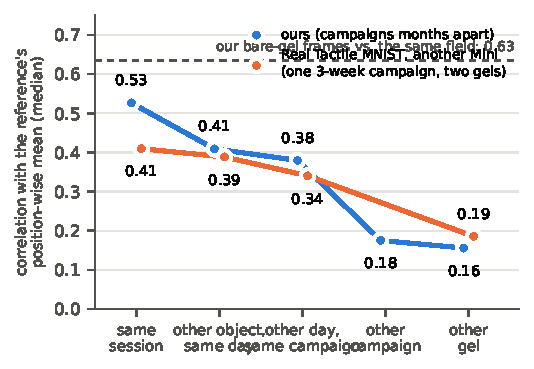
\includegraphics[width=\linewidth]{fig/fig_day_signature.pdf}
  \caption{\textbf{Contact images carry a day signature of the sensor.} Median correlation between the fine band (190--370\,\si{\micro\metre}) of a contact image and the position-wise mean of other contacts, as a function of how the reference relates to the contact. On our sensor (blue, 55 sessions over four months) a contact matches other \emph{objects} touched the same day almost as well as other contacts of its own session, and barely matches another day or the other gel. The same ordering appears on another lab's GelSight Mini (orange, Real Tactile MNIST~\cite{tactilemnist2025}, 24 runs over 15 days). Our no-contact frames do not contain the pattern (dashed).}
  \label{fig:signature}
\end{figure}

We recorded 2{,}711 grasps of 20 materials with one GelSight Mini over four months, in four campaigns separated by weeks, with the normal force co-recorded by a force sensor on the opposing finger, and, in the last campaign, bare-gel frames before and between grasps. Holding out the last campaign reveals a failure that no cross-unit study predicts. A supervised encoder trained in June--July recognises materials in September--October at \SupFoneRawSAcc\pct\ (chance 5\pct) and assigns \SupFoneRawSTop\pct\ of all episodes to a single class; frozen Sparsh encoders~\cite{higuera2024sparsh}, pretrained on GelSight Mini data, do no better (\SdinoRawAcc--\IjepaRawAcc\pct).

The cause is measurable without any model (\cref{fig:signature}). At a fixed image position, the fine-scale content of a contact image correlates with the average of \emph{other objects touched the same day} at \SigSameDay\ (median over sessions), almost as much as with the same session's other contacts (\SigOwn), and only at \SigOtherEra\ with another day's. The pattern is broadband, is strongest on rigid samples that cannot transmit a backing, and is \emph{absent from no-contact frames} (\num{0.06}): it is a property of the loaded gel on that day. Because a recording session holds one object, any material classifier can satisfy its labels with the day signature, and does; an era classifier applied to June contacts re-rendered under a July sensor state calls them July (\cref{sec:signature}).

This paper makes four contributions.
\textbf{(1)} We measure the day signature and its drift mechanisms---slow with use, a step at every power-up, a reset at gel replacement---on 620 bare-gel frames and 55 sessions, and replicate the signature on a second unit in public data.
\textbf{(2)} We show that the signature is the shortcut: every encoder we test collapses on a later day, and the standard fix, batch-norm re-estimation per session, collapses to chance because a session holds one object; on a public dataset whose runs hold all objects it works, confirming the mechanism.
\textbf{(3)} We separate sensor state from touch using only the robot's own contact stream. The \emph{loaded state}, the position-wise mean of recent contacts, is subtracted at test time (every encoder recovers: frozen Sparsh \num{3}$\times$, a supervised CNN \SupFoneRawSAcc$\rightarrow$\SupFonePrevSAcc\pct, and \SupAugFonePrevSAcc\pct\ with standard photometric jitter) or used at training time: re-rendering training contacts under other sessions' states and contrasting against position-matched decoys trains, with no labels and no test-time data, a small adapter that lifts frozen Sparsh-I-JEPA from \IjepaRawAcc\ to \IjepaAdAcc\pct.
\textbf{(4)} We show which cues survive: normal force read as marker spreading against the \emph{unloaded} gel transfers across months ($r$=\ForceGeomXeraC), where every appearance-based force estimate fails ($R^2\le\ForceLearnedBestR$); contact detection needs the same unloaded reference. The picture that emerges is a state-aware decomposition rather than one more invariant network: appearance needs the loaded state removed, geometry needs the unloaded state, and both states come from the stream the robot already produces.

\section{Related work}
\label{sec:related}

\paragraph{Tactile representations and their evaluation.}
Self-supervised tactile encoders are trained on large frame collections: Sparsh~\cite{higuera2024sparsh}, T3~\cite{t3fota2024}, UniTouch~\cite{unitouch2024}, AnyTouch~\cite{anytouch2025,anytouch2026two} and the TVL data~\cite{tvl2024}. TactSpace aligns several views of one contact in a shared latent space~\cite{tactspace2026}. These models are evaluated inside the collection they were trained on, with random or object-level splits. RCT shows that frame-level splits of TVL leak the sequence and that a held-out DIGIT is a separate difficulty~\cite{rct2026}, and a recent material benchmark on TVL's HCT data still shares sessions between training and test~\cite{mohsan2026language}. The sensor enters as preprocessing: Sparsh, SITR, AnyTouch~2 and HTT subtract a background frame~\cite{higuera2024sparsh,sitr2025,anytouch2026two,htt2026}, and UniTouch adds a token for the sensor type~\cite{unitouch2024}. GelSlim re-captures its blank frame every hundred grasps and tracks image quality over 3{,}300 grasps~\cite{gelslim2018}, and other work measures how the unloaded image degrades with load cycles~\cite{davis2025resilience,cottrell2026durable}. None of these studies holds out hardware of the same model over months or tests what the background frame removes.

\paragraph{Transfer across units and gels.}
That units of one model differ is well documented. SITR combines background subtraction, 18 calibration presses per unit and a million simulated images, and reaches 90\pct\ when a 16-object classifier is moved between four GelSight Minis, against 73\pct\ for an ImageNet ViT~\cite{sitr2025}. BIDETA adapts frozen Sparsh to sibling units with labelled target contacts~\cite{bideta2026}. TacVerse benchmarks seven sensors with chronological splits inside one campaign~\cite{tacverse2026}. FEATS and FeelAnyForce find that force estimates degrade on a new unit or gel~\cite{feats2025,feelanyforce2024}. Others translate between sensors conditioned on the target's blank frame~\cite{genforce2026,castano2026forcemap,split2026} or align different sensor types~\cite{cttp2024,htt2026}. Each of these methods needs blank frames, calibration presses, simulation or target labels. Our estimate needs only the robot's ordinary contacts.

\paragraph{Test-time adaptation and change detection.}
Adapting to a shifted test distribution without labels is usually done by re-estimating normalisation statistics (AdaBN~\cite{li2018adabn}), by minimising prediction entropy (TENT~\cite{wang2021tent}), or by re-estimating class priors~\cite{saerens2002labelshift}. These methods assume mixed batches. When the stream is ordered by object, as a robot's stream is, normalisation statistics absorb the object~\cite{burns2021bn}, and dedicated methods handle temporal correlation~\cite{gong2022note,boudiaf2022lame}. Our detector is a two-window test in the tradition of sequential change detection~\cite{page1954cusum}, applied to image statistics that we chose because they separate a change of hardware from a change of object.

\paragraph{Acquisition shortcuts and flat-fields from the data.}
Classifiers that learn the hospital from a radiograph~\cite{zech2018hospital}, the acquisition setup from a COVID study~\cite{degrave2021covid}, the scanner from an MRI~\cite{fortin2017combat} or the dataset from a photograph~\cite{torralba2011bias,liuhe2025} are instances of shortcut learning~\cite{geirhos2020shortcut}, and our finding is the tactile instance. Removing batch information by gradient reversal does not improve generalisation there~\cite{sypetkowski2023rxrx1}. Microscopy estimates an illumination field from the image collection itself, as the per-pixel mean of a batch~\cite{singh2014illumination} or its low-rank refinement~\cite{peng2017basic}, and infrared imaging does the same for fixed-pattern noise~\cite{harris1999nuc}. The same averaging identifies a camera by its sensor noise~\cite{lukas2006prnu}. Our estimate is such a flat-field, taken from a robot's stream of contacts and restarted when the hardware changes.

\section{The hardware state in a tactile image}
\label{sec:signature}

\paragraph{Data.}
A GelSight Mini (1640$\times$1232 native frames, \SI{11.3}{\micro\metre}/px, \SI{18.8}{fps}, printed markers) is mounted on one finger of a parallel gripper, and an ATI Nano17 on the other finger measures the normal force. The object is a box whose face carries one of 20 materials. It is clamped in a fixture with foam behind it so that the contact aligns itself. Each episode grasps the face at one of two forces (40 or 80\pct\ of a per-material maximum, 0.9--5\,N) and strokes it by 2\,cm in four directions and a circle. The gel is lubricated every five episodes, and one session records one material. Four campaigns cover four months: A (June 15--22), B (July 6--8), C (July 9--13) and D (September 22 to October 15), \EpRecorded\ episodes in all. \EpNoCrops\ episodes of campaign D have no eight-frame span of contact inside the stroke, so the material experiments use \EpCrops. Two units and three gels were used. Unit 1 carried gel 1 until July 9, unit 2 carried gel 2 from July 10, and gel 3 replaced gel 2 on October 9 between 18:42 and 19:37. We call these three combinations hardware states S1, S2 and S3. The laboratory log recorded a change of unit and four gel replacements. The images show exactly the two changes above, and the operators confirmed them against their notes. Campaign D also records frames of the bare gel. The camera's exposure and white balance are fixed: on a held contact the mean of each colour channel drifts by at most 0.3 grey levels per episode. We never resample a frame. Material models read native 192-px crops.

\paragraph{Measurement.}
For every session we form the position-wise mean of its contact crops in frame coordinates, its \emph{state field} $F_s(p)$. For a sampled contact crop we correlate its fine band (190--370\,\si{\micro\metre}) with the same band of another session's field, excluding pixels within 60\,px of a printed marker so that inpainting residue cannot contribute. \Cref{fig:signature} shows the medians over sessions. A contact matches its own session's other contacts at \HwFarOwn, another object touched the same day at \HwFarSameDay, the same unit and gel on another day at \HwFarWeeks, and the same unit and gel three months later at \HwFarMonths. It does not match the other unit (\HwFarOtherUnit) or the other gel of the same unit (\HwFarOtherGel). Frames of the bare gel, with nothing touching it, match their session's contact field at \BlankVsFieldFar. Another lab's GelSight Mini shows the same ordering~\cite{tactilemnist2025}, although its correlation across a gel swap stays higher (\TmSigOtherGel).

\paragraph{What the state is.}
The pattern appears to be fixed relative to the camera. Warping a bare-gel frame by the membrane's measured displacement lowers its match to the session field from \BlankVsFieldFar\ to \WarpedBlankVsFieldFar. The membrane moves by a median of only \WarpDispPx\,px, however, so this test is weak. It is nevertheless carried by the gel cartridge, because a new gel on the same unit and camera removes it. We therefore read it as an optical property of the cartridge seen through the camera, rather than as texture on the deforming surface. The state also has a smooth part, the illumination field, which changes a little from session to session on the same hardware. Between two bare-gel frames of one session, the illumination moves by a median \DriftUse\ grey levels over \DriftUseContacts\ grasps. Between the last bare-gel frame of one session and the first of the next, with no contact in between, it moves by \DriftIdle. A contact matches its own session (\HwFarOwn) better than another object touched the same day (\HwFarSameDay) because the session's mean contains the same object. Within one unit and gel, a session's illumination field lies \LpDistWithinSthree--\LpDistWithinSone\ grey levels from the mean of its hardware state. The two units differ by \LpDistSoneStwo\ grey levels, and the two gels on unit 2 by \LpDistStwoSthree.

\paragraph{The images record the hardware history.}
The changes are sharp enough to date from the images alone. Correlating every pair of the 35 June and July sessions splits them into two blocks at July 9 to 10 and nowhere else, and the September and October sessions split at October 9. This is how we established the timeline above, which the laboratory log had recorded wrongly. \Cref{sec:tracker} turns the same observation into a detector that runs while the robot works.

\section{Separating sensor state from touch}
\label{sec:method}

We model a contact image at position $p$ in session $s$ as $x = F_s(p) + r$: the sensor's loaded state at that position on that day, plus a contact-specific residual that carries the surface. $F_s$ is estimated from the stream the robot already produces---the position-wise mean of contacts---with no labels, blank frames, calibration presses or simulator. Three uses follow.

\paragraph{Stream calibration (test time).}
Replace the current state by the training mean: $\tilde{x} = x - \hat F(p) + G(p)$, with $G$ the mean field over training sessions. The deployable choice of $\hat F$ is the field of the \emph{previous} session---a different object, hence carrying no information about the current one---optionally updated online with every new contact. We also report the optimistic source (the current session's other contacts) and the dependence on how many contacts have been seen.

\paragraph{State swap (training time, label-free).}
Each training contact is re-rendered under another session's state, $x' = r + F_{s'}(p)$, and an encoder $f$ is trained to match $f(x)$ and $f(x')$ with InfoNCE~\cite{oord2018cpc,chen2020simclr}. Two details matter. Batches are built from a few sessions so that negatives share the anchor's state, and \emph{decoy} negatives are added: another contact's residual placed at the anchor's position under the anchor's state, $x^{d} = r_{j} + F_s(p)$, so that the only way to tell the positive from the decoy is the surface. Sessions and image positions are recording metadata; no material label enters the objective. (The gain from the decoys is measured in \cref{sec:ablation}.)

\paragraph{State-swap adapter on a frozen foundation model.}
The same objective trains a two-layer MLP on top of a frozen tactile foundation model (Sparsh~\cite{higuera2024sparsh}, 768-d tokens mean-pooled); the encoder's own two-frame input is re-rendered on both frames. Training takes twelve minutes on one GPU and needs neither labels nor any data from the deployment day.

\paragraph{The unloaded state for geometry and contact.}
Normal force and contact are not appearance quantities. We read them against the \emph{unloaded} gel, the bare-gel frames the robot sees between grasps: for force, the marker grid detected on the bare gel at native resolution is matched to the grid in a contact frame, and the affine summary of the displacement field (divergence, mean displacement, net shear) is mapped to force by a linear map; for contact, a detector operates on $f(x) - f(\text{bare gel of the session})$. \Cref{sec:force,sec:contact} show that the force reference only needs refreshing at a gel swap (a new gel has a new stiffness), whereas the appearance state drifts daily.

\section{Experiments}
\label{sec:exp}

\paragraph{Protocol.}
The main split trains on campaigns A, B and C (June and July, \EpTrainABC\ episodes) and tests on campaign D (September and October, \EpTestD\ episodes, 20 materials, chance 5\pct). The test set holds three hardware relations. Fifteen materials were learned on unit 1 and are tested on unit 2, a different unit and gel. Four rigid materials (cork, fibreglass, ABS, ceramic) were learned on unit 2 in July and are tested on its replaced gel. Wood was learned on unit 1 and is tested on the replaced gel of unit 2. Two of the fifteen materials, textured rubber and EPDM foam, were replaced by new pieces of the same kind before campaign D. Every CNN input is a single native 192-px crop, twelve per episode, and the logits of an episode's crops are summed. We report macro accuracy, macro-F1, and the share of test episodes assigned to the most predicted class, which exposes a collapse onto few classes. The CNN is a four-stage convolutional encoder at native resolution. Its input is the colour crop plus two band-pass detail images and two high-passed log colour ratios. Each stage applies two $3\times3$ convolutions with BatchNorm and GELU and then downsamples with anti-aliasing. It is trained with cross-entropy for 12 epochs with AdamW. Its jitter variant adds per-channel gains ($\pm$20\pct) and a smooth multiplicative field ($\pm$15\pct) during training. Heads are MLPs on frozen embeddings with three seeds, and CNN numbers average three training seeds. Rows that subtract a state estimate read the training images relative to their own previous session, so that the head sees the same transform at training and test time. All other rows read the training images raw. Sparsh~\cite{higuera2024sparsh} receives its own two-frame input (two frames of the crop, five apart) and DINOv2~\cite{oquab2024dinov2} the mean of eight consecutive frames. All design choices were made on this split, and the other three campaign folds in \cref{sec:timeorstate} are independent of them.

\begin{table}[t]
  \centering\footnotesize\setlength{\tabcolsep}{3pt}
  \caption{\textbf{Material after a change of hardware.} Train June--July, test September--October (20 materials, chance 5\pct). All: accuracy\,/\,macro-F1. Other unit: the 15 materials learned on unit~1. Other gel: the 4 learned on unit~2 before its gel was replaced. Top: share of episodes in the most predicted class. Non-causal rows use test data that a robot would not yet have.}
  \label{tab:material}
  \resizebox{\linewidth}{!}{%
  \begin{tabular}{@{}lcccc@{}}
    \toprule
    reading of the test images & all & other unit & other gel & top \\
    \midrule
    \multicolumn{5}{@{}l}{\emph{CNN}} \\
    raw & \af{\SrcSupNoneAcc}{\SrcSupNoneF} & \DOneSupRaw & \DTwoSupRaw & \SrcSupNoneTop \\
    \ \ label-shift correction~\cite{saerens2002labelshift} & \af{\TtaSupLabelshiftAcc}{\TtaSupLabelshiftF} & \DOneTtaSupLabelshift & \DTwoTtaSupLabelshift & \TtaSupLabelshiftTop \\
    \ \ TENT, online~\cite{wang2021tent} & \af{\TtaSupTentAcc}{\TtaSupTentF} & \DOneTtaSupTent & \DTwoTtaSupTent & \TtaSupTentTop \\
    \ \ TENT, mixed batches (non-causal) & \af{\TtaSupTentIidAcc}{\TtaSupTentIidF} & \DOneTtaSupTentIid & \DTwoTtaSupTentIid & \TtaSupTentIidTop \\
    \ \ AdaBN per hardware state, causal & \af{\TtaSupAdabnCausalAcc}{\TtaSupAdabnCausalF} & \DOneTtaSupAdabnCausal & \DTwoTtaSupAdabnCausal & \TtaSupAdabnCausalTop \\
    \ \ AdaBN per hardware state (non-causal)~\cite{li2018adabn} & \af{\TtaSupAdabnEpochsAcc}{\TtaSupAdabnEpochsF} & \DOneTtaSupAdabnEpochs & \DTwoTtaSupAdabnEpochs & \TtaSupAdabnEpochsTop \\
    \ \ $-$ previous session's state & \af{\SrcSupPrevAcc}{\SrcSupPrevF} & \DOneSupPrev & \DTwoSupPrev & \SrcSupPrevTop \\
    \ \ $-$ the session's bare gel & \af{\SrcSupBlankAcc}{\SrcSupBlankF} & \DOneSupBlank & \DTwoSupBlank & \SrcSupBlankTop \\
    \ \ $-$ \cref{alg:tracker} & \textbf{\af{\SrcSupTrkFrAcc}{\SrcSupTrkFrF}} & \DOneSupTrkFr & \DTwoSupTrkFr & \SrcSupTrkFrTop \\
    \midrule
    \multicolumn{5}{@{}l}{\emph{CNN trained with photometric jitter}} \\
    raw & \af{\SrcAugNoneAcc}{\SrcAugNoneF} & \DOneAugRaw & \DTwoAugRaw & \SrcAugNoneTop \\
    \ \ AdaBN per hardware state (non-causal) & \af{\TtaAugAdabnEpochsAcc}{\TtaAugAdabnEpochsF} & \DOneTtaAugAdabnEpochs & \DTwoTtaAugAdabnEpochs & \TtaAugAdabnEpochsTop \\
    \ \ TENT, mixed batches (non-causal) & \af{\TtaAugTentIidAcc}{\TtaAugTentIidF} & \DOneTtaAugTentIid & \DTwoTtaAugTentIid & \TtaAugTentIidTop \\
    \ \ $-$ previous session's state & \af{\SrcAugPrevAcc}{\SrcAugPrevF} & \DOneAugPrev & \DTwoAugPrev & \SrcAugPrevTop \\
    \ \ $-$ \cref{alg:tracker} & \textbf{\af{\SrcAugTrkFrAcc}{\SrcAugTrkFrF}} & \DOneAugTrkFr & \DTwoAugTrkFr & \SrcAugTrkFrTop \\
    \midrule
    \multicolumn{5}{@{}l}{\emph{Frozen foundation encoders}} \\
    Sparsh-I-JEPA, raw & \af{\IjepaRawAcc}{\IjepaRawF} & \DOneIjepaRaw & \DTwoIjepaRaw & \IjepaRawTop \\
    \ \ $-$ previous session's state & \af{\IjepaPrevAcc}{\IjepaPrevF} & \DOneIjepaPrev & \DTwoIjepaPrev & \IjepaPrevTop \\
    \ \ $-$ \cref{alg:tracker} & \textbf{\af{\IjepaTrkFrAcc}{\IjepaTrkFrF}} & \DOneIjepaTrkFr & \DTwoIjepaTrkFr & \IjepaTrkFrTop \\
    Sparsh-DINO, raw & \af{\SdinoRawAcc}{\SdinoRawF} & \DOneSdinoRaw & \DTwoSdinoRaw & \SdinoRawTop \\
    \ \ $-$ \cref{alg:tracker} & \af{\SdinoTrkFrAcc}{\SdinoTrkFrF} & \DOneSdinoTrkFr & \DTwoSdinoTrkFr & \SdinoTrkFrTop \\
    Sparsh-MAE, raw & \af{\MaeRawAcc}{\MaeRawF} & \DOneMaeRaw & \DTwoMaeRaw & \MaeRawTop \\
    \ \ $-$ \cref{alg:tracker} & \af{\MaeTrkFrAcc}{\MaeTrkFrF} & \DOneMaeTrkFr & \DTwoMaeTrkFr & \MaeTrkFrTop \\
    DINOv2, raw & \af{\DinovRawAcc}{\DinovRawF} & \DOneDinovRaw & \DTwoDinovRaw & \DinovRawTop \\
    \ \ $-$ previous session's state & \af{\DinovPrevAcc}{\DinovPrevF} & \DOneDinovPrev & \DTwoDinovPrev & \DinovPrevTop \\
    \bottomrule
  \end{tabular}}
\end{table}

\subsection{What a change of hardware does to a classifier}
\label{sec:material}

\Cref{tab:material} gives the main result. Read raw, the CNN scores \SrcSupNoneAcc\pct\ and puts \SrcSupNoneTop\pct\ of all test episodes into a single class, one of the four materials it saw on unit 2. The fifteen materials it learned on unit 1 score \DOneSupRaw\pct. The four materials learned on unit 2 score \DTwoSupRaw\pct, mostly because the classifier sends many episodes to them. Frozen Sparsh encoders show the same collapse. The jitter CNN collapses much less. It scores \SrcAugNoneAcc\pct, puts \SrcAugNoneTop\pct\ of the episodes in one class, and reaches \DOneAugRaw\pct\ on the cross-unit materials.

Reading the images relative to the state undoes the collapse. With \cref{alg:tracker}, the CNN reaches \SrcSupTrkFrAcc\pct\ and the cross-unit materials \DOneSupTrkFr\pct. This lies between the previous session's state (\SrcSupPrevAcc\pct) and a bare-gel frame of the same session (\SrcSupBlankAcc\pct). Those two sources are picked by hand, while the tracker chooses its source and restarts by itself. Frozen Sparsh-I-JEPA rises from \IjepaRawAcc\ to \IjepaTrkFrAcc\pct, and the other Sparsh encoders gain as well. On the four materials that cross the gel replacement, the reading halves the accuracy for every encoder: from \DTwoSupRaw\ to \DTwoSupTrkFr\pct\ for the CNN, from \DTwoAugRaw\ to \DTwoAugTrkFr\pct\ for the jitter CNN and from \DTwoIjepaRaw\ to \DTwoIjepaTrkFr\pct\ for Sparsh-I-JEPA. The collapse explains part of their raw score, but not for the jitter CNN, which collapses only mildly (\cref{sec:timeorstate}).

The adaptation baselines do not fix the collapse. Label-shift correction re-estimates the class priors from the test predictions. It finds that the class receiving most episodes is frequent, and it makes the collapse worse. Online TENT, which updates on one object at a time as a robot would, collapses entirely, and AdaBN per hardware state reaches \TtaSupAdabnEpochsAcc\pct\ even with the true change dates and all of the state's test images. Both methods assume that a batch mixes classes, and one object per session violates this assumption~\cite{burns2021bn}. Given mixed batches that a robot would not have, TENT reaches \TtaSupTentIidAcc\pct. We did not run methods designed for temporally correlated streams~\cite{gong2022note,boudiaf2022lame}. For the jitter CNN, every adaptation baseline is below its raw score, and only the state estimate improves it.

An adapter trained on the same decomposition without material labels lifts frozen Sparsh-I-JEPA less than the reading does (\IjepaAdAcc\pct, supplement).

\subsection{The tracker on the stream}
\label{sec:trackerexp}

\begin{figure}[t]
  \centering
  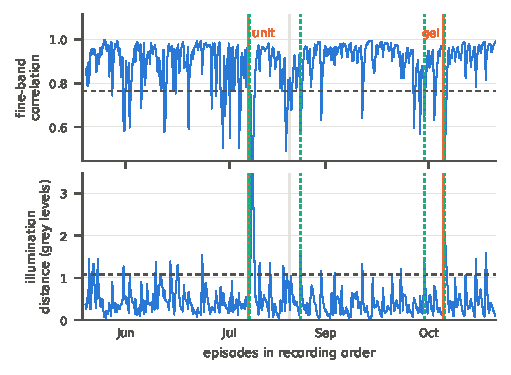
\includegraphics[width=\linewidth]{fig/fig_tracker.pdf}
  \caption{\textbf{\Cref{alg:tracker}'s detector over four months}, \EpRecorded\ episodes in recording order, on whole frames. Top: fine-band correlation between the last 8 episodes and the 30 before them. Bottom: distance between their illumination fields. Dashed: thresholds from the first hardware state. Orange: the change of unit and the gel replacement. Green: alarms (two false). Grey: the summer break.}
  \label{fig:tracker}
\end{figure}

\begin{table}[t]
  \centering\footnotesize\setlength{\tabcolsep}{3.5pt}
  \caption{\textbf{Detecting a change of hardware} with thresholds fixed in advance (10th and 95th percentiles of the two statistics on one unit of each dataset, $m\!=\!5$). Streams splice recordings of one unit or gel onto another (100 streams) or onto other recordings of the same hardware (100 streams). SITR: changes between two Minis only. Delay and false alarms are counted in the dataset's items.}
  \label{tab:detect}
  \resizebox{\linewidth}{!}{%
  \begin{tabular}{@{}llccc@{}}
    \toprule
    dataset & changes & detected & delay & false alarms \\
    & & (\pct) & (median) & per 1{,}000 \\
    \midrule
    ours, whole frames (episodes) & unit, gel & \TeOursFramesDet & \TeOursFramesDelay & \TeOursFramesFa \\
    ours, material crops (episodes) & unit, gel & \TeOursDet & \TeOursDelay & \TeOursFa \\
    SITR~\cite{sitr2025} (images) & Mini to Mini & \TeSitrMiniDet & \TeSitrMiniDelay & \TeSitrFa \\
    FEATS~\cite{feats2025} (images) & unit, gel & \TeFeatsDet & \TeFeatsDelay & \TeFeatsFa \\
    Tactile MNIST~\cite{tactilemnist2025} (touches) & gel & \TeTmnistDet & \TeTmnistDelay & \TeTmnistFa \\
    \bottomrule
  \end{tabular}}
\end{table}

Run over all \EpRecorded\ episodes in recording order (\cref{fig:tracker}), the detector raises \FrAlarms\ alarms. One comes \FrUnitLatency\ episodes after the change of unit and one \FrGelLatency\ episodes after the gel replacement. The other \FrFalseAlarms\ are false: one in the second September session, after the summer break, and one the day before the gel replacement. With stricter thresholds, the 1st and 99th percentiles, it detects both changes later (\FrSweepOneUnit\ and \FrSweepOneGel\ episodes) and raises no false alarm (supplement). A canvas session, whose weave lowers the fine correlation, and the illumination steps between sessions raise no alarm, because they do not occur together. \Cref{tab:detect} applies the same rule to streams spliced from four datasets, with thresholds set on one unit of each and nothing tuned on change points. It detects \TeOursFramesDet\pct\ of the changes spliced from our recordings: \TeOursFramesUnitDet\pct\ of those that involve the other unit, and \TeOursFramesGelDet\pct\ of the gel changes on the same unit. On the public datasets it detects \TePubDetMin--\TePubDetMax\pct, with \TePubFaMax\ or fewer false alarms per 1{,}000 items everywhere. Whole frames matter. Our first implementation computed the statistics on the material crops, which cover each frame sparsely, so that a window holds one object seen through a few crops per pixel. On the real stream it missed the change of unit, and on spliced streams it detected only \TeOursDet\pct\ of the changes. A per-object variant on the crops did no better (supplement). We moved to whole frames after these failures and kept the rule, so the real-stream result above is not an independent test, while the spliced public streams are.

Detecting the changes matters. A running mean that is never restarted reaches \SrcSupNoResetAcc\pct\ for the CNN. The crop-based detector missed the change of unit, so its estimate for the September sessions still averaged objects seen on the first unit, and the CNN reached \SrcSupTrkAcc\pct. With the whole-frame detector's restarts it reaches \SrcSupTrkFrAcc\pct. Started at the deployment in September, the reading gives \SrcSupTrkFrDepAcc\pct\ with the two false alarms and \SrcSupTrkDepAcc\pct\ with a single restart at the gel replacement, so the false alarms cost nothing measurable.

\subsection{What the estimate needs}
\label{sec:sources}

\begin{table}[t]
  \centering\footnotesize\setlength{\tabcolsep}{4pt}
  \caption{\textbf{Which estimate of the state} (accuracy on campaign D, three seeds). Every estimate uses unlabelled frames of the deployment.}
  \label{tab:sources}
  \begin{tabular}{@{}lcc@{}}
    \toprule
    estimate $\hat F$ subtracted from the test image & CNN & + jitter \\
    \midrule
    none & \SrcSupNoneAcc & \SrcAugNoneAcc \\
    previous session, mean in feature space & \SrcSupFeatAcc & \SrcAugFeatAcc \\
    previous session, mean colour only & \SrcSupMeancolAcc & \SrcAugMeancolAcc \\
    previous session, smooth illumination only & \SrcSupLowpassAcc & \SrcAugLowpassAcc \\
    previous session, full field & \SrcSupPrevAcc & \SrcAugPrevAcc \\
    own session's other contacts (same object) & \SrcSupOwnAcc & \SrcAugOwnAcc \\
    a random other session of the campaign & \SrcSupRandAcc & \SrcAugRandAcc \\
    all sessions of the campaign (non-causal) & \SrcSupCampAcc & \SrcAugCampAcc \\
    the session's bare gel & \SrcSupBlankAcc & \SrcAugBlankAcc \\
    \cref{alg:tracker} (causal, automatic restarts) & \SrcSupTrkFrAcc & \SrcAugTrkFrAcc \\
    \bottomrule
  \end{tabular}
\end{table}

\Cref{tab:sources} varies only the test-time estimate. Any unlabelled frames of the deployment work, provided they come from other objects: the previous session, a random other session, all sessions together, or the bare gel. The session's own contacts are the worst full-field estimate, because their mean contains the object. The number of objects matters more than the number of contacts. In a separate run with one seed, an estimate built from one other object gives \CvSupObjOne\pct, from two objects \CvSupObjTwo\pct\ and from nineteen \CvSupObjNineteen\pct. For the CNN, the smooth illumination field alone does as well as the full field (\SrcSupLowpassAcc\ against \SrcSupPrevAcc\pct). For the jitter CNN the fine pattern adds about four points (\SrcAugLowpassAcc\ against \SrcAugPrevAcc\pct). A single colour per session recovers part of the gain, and centring the features does not work. The bare gel works as well as the contacts, so standard flat-fielding is a valid estimate of the state where blank frames exist. The contact stream gives the same estimate where they do not, which is the case for archived datasets and for our training campaigns.

\subsection{Where the correction helps}
\label{sec:timeorstate}

\begin{table}[t]
  \centering\footnotesize\setlength{\tabcolsep}{3.5pt}
  \caption{\textbf{Each campaign held out in turn} (accuracy, 20-way). A and B are tested on hardware seen in training for every test material. In C, four test materials were learned on the other gel and wood on the other unit. D is the split of \cref{tab:material}. Folds A--C: one training seed.}
  \label{tab:rotation}
  \begin{tabular}{@{}lcccc@{}}
    \toprule
    test campaign & A & B & C & D \\
    \midrule
    CNN, raw & \FoldASupRawAcc & \FoldBSupRawAcc & \FoldCSupRawAcc & \SrcSupNoneAcc \\
    \ \ $-$ previous session's state & \FoldASupPrevAcc & \FoldBSupPrevAcc & \FoldCSupPrevAcc & \SrcSupPrevAcc \\
    CNN + jitter, raw & \FoldAAugRawAcc & \FoldBAugRawAcc & \FoldCAugRawAcc & \SrcAugNoneAcc \\
    \ \ $-$ previous session's state & \FoldAAugPrevAcc & \FoldBAugPrevAcc & \FoldCAugPrevAcc & \SrcAugPrevAcc \\
    Sparsh-I-JEPA, raw & \FoldAIjepaRawAcc & \FoldBIjepaRawAcc & \FoldCIjepaRawAcc & \IjepaRawAcc \\
    \ \ $-$ previous session's state & \FoldAIjepaPrevAcc & \FoldBIjepaPrevAcc & \FoldCIjepaPrevAcc & \IjepaPrevAcc \\
    \bottomrule
  \end{tabular}
\end{table}

\Cref{tab:rotation} holds out each campaign in turn. Time alone is not the problem. Sessions recorded weeks apart on the hardware seen in training are recognised at \FoldBSupRawAcc--\FoldASupRawAcc\pct\ raw (folds A and B), and the state itself changes little over three months. Its fine band still correlates at \HwFarMonths, against \HwFarWeeks\ after weeks, and its illumination field has moved by \LpDistStwoJulSep\ grey levels. Within known states the subtraction is unnecessary and can cost up to \num{10} points, because the training mean $G$ is then a mixture of states that no real session has. The gain in fold D is a gain against a collapse, and the collapse comes from the training set. Trained on A and B alone, which hold fifteen materials, all on unit 1, the CNN collapses less on D (\TsABSupRawAcc\pct\ raw over all 20 test materials, at most 75\pct\ possible, with \TsABSupRawTop\pct\ in one class). The state estimate adds less (\TsABSupPrevAcc\pct), and the jitter CNN gains nothing from it (\TsABAugRawAcc\ against \TsABAugPrevAcc\pct). Trained on A and C, with four materials again recorded only on unit 2, it collapses again (\TsACSupRawAcc\pct) and recovers to \TsACSupPrevAcc\pct. Trained on June alone, it scores \GapFoneSupBRawAcc\pct\ on its fifteen materials weeks later on the same unit and \GapFoneSupDRawAcc\pct\ on the other unit, and the estimate does not recover that loss (\GapFoneSupDPrevAcc\pct). The estimate therefore repairs the shortcut that one session per object creates, and it does not repair everything a change of hardware costs.

Two cases are not repaired. In fold C, all five test materials were learned on gel 3 only and are tested on earlier hardware. The four rigid materials score \FoldCSupRawFour\pct\ raw and \FoldCSupPrevFour\pct\ with the state removed, wood scores \FoldCSupRawWood\ and \FoldCSupPrevWood\pct, and frozen Sparsh is at chance. In fold D, the same four materials cross the gel replacement in the other direction, and the reading halves their accuracy. Wood, which crosses both unit and gel in fold D, is recovered there. Both failures involve the gel replacement. The change of unit also replaced a gel and was corrected, however, and the four materials are rigid and were recorded in a single session per gel. All sessions on the replaced gel hold these materials, so we cannot separate the gel, the materials and the training-set structure as the cause.

\subsection{Other sensors and the hardware in foundation features}
\label{sec:second}

\paragraph{Foundation features encode the unit.}
Fourteen materials were recorded on both units. A linear probe trained on frozen features of some of these materials, and tested on the others, tells the two units apart from a single crop at \ProbeSdinoRawUnit\pct\ for Sparsh-DINO, \ProbeIjepaRawUnit\ for Sparsh-I-JEPA, \ProbeDinovRawUnit\ for DINOv2 and \ProbeCnnRawUnit\ for our CNN, where chance is 50\pct. Read relative to the previous session's state, the same crops give \ProbeSdinoPrevUnit, \ProbeIjepaPrevUnit, \ProbeDinovPrevUnit\ and \ProbeCnnPrevUnit\pct, while the material probe on the same features drops by one to six points (supplement). The two units were also used in different seasons, which this probe cannot separate from the hardware.

\paragraph{SITR: four GelSight Minis.}
SITR's released classification set has 20 objects pressed on seven sensors, four of them GelSight Minis~\cite{sitr2025}. Following its protocol with a frozen DINOv2, a head trained on one Mini scores \SitrDinovRawIntra\pct\ on the other three raw, \SitrDinovBgIntra\pct\ with SITR's background image subtracted, and \SitrDinovStreamIntra\pct\ relative to the mean of the sensor's own unlabelled images. That mean uses the 16{,}000 images of the sensor's training split, and the test images are not among them. The mean of 100 random images gives \SitrDinovStreamHundredIntra\pct, and the mean of 20 is worse than no correction (\SitrDinovStreamTwentyIntra\pct), because it still contains the objects in those 20 presses. The stream estimate thus needs many images, while SITR needs 18 calibration presses per sensor. The hardware remains decodable after the correction (probe \SitrDinovStreamProbe\pct), and the reading does little for our CNN (\SitrCnnRawIntra\ to \SitrCnnStreamIntra\pct) or for Sparsh (\SitrIjepaRawIntra\ to \SitrIjepaStreamIntra\pct, supplement). SITR itself reports 90\pct\ on its 16-object version with calibration presses and simulated pretraining, and 73\pct\ for an ImageNet ViT.

\paragraph{FEATS: force across units and gels.}
FEATS records indenters with known force maps on five Minis and six gels~\cite{feats2025}. A linear probe on its labelled no-contact frames identifies both the sensor and the gel at \FeatsProbeSensor\pct, so the state is in the bare frame there as well. A CNN regressing normal force reaches \FeatsRawTestMae\,N on the training hardware and \FeatsRawOldGelMae\,N and \FeatsRawNewGelMae\,N on another unit with its old and a new gel. Relative to the stream estimate the errors are \FeatsStreamOldGelMae\ and \FeatsStreamNewGelMae\,N, and relative to the no-contact frame \FeatsBgOldGelMae\ and \FeatsBgNewGelMae\,N. No image-space reading brings force across hardware close to the training error.

\paragraph{Real Tactile MNIST: a gel swap on another lab's sensor.}
On Real Tactile MNIST (a digit from single touches, 24 runs over three weeks, one gel swap)~\cite{tactilemnist2025}, frozen Sparsh-I-JEPA collapses on later runs whether or not the gel was swapped, with \TmLaterIjepaRawTop\pct\ of the touches in one class on the same gel and \TmGelIjepaRawTop\pct\ after the swap. Reading relative to the previous run's state reduces the collapse in both cases and lifts accuracy from \TmLaterIjepaRawAcc\ to \TmLaterIjepaPrevAcc\pct\ and from \TmGelIjepaRawAcc\ to \TmGelIjepaPrevAcc\pct. The data therefore show the shortcut but do not tie it to the gel swap. For the supervised model, per-run AdaBN does better than the state reading (\TmGelSupAdaRunAcc\ against \TmGelSupPrevAcc\pct\ after the swap), because every run contains all ten digits. This is the mixed-class condition that our one-object sessions lack.

\subsection{Normal force}
\label{sec:force}
Force is a matter of mechanics, and the state does not describe it. Whole-frame models trained on June and July to regress normal force from appearance reach $R^2\le\ForceLearnedBestR$ on September and October, even with the state removed. Marker spreading measured against a bare-gel marker grid transfers better. June and July have no bare-gel frames, so their marker displacements are referenced to a bare-gel grid recorded in September. A linear map of three affine statistics of the displacement field, fitted on June and July, then predicts the September and October sessions before the gel replacement at $r=\ForceGeomXeraC$ ($R^2=\ForceGeomXeraR$), and the reverse fit predicts June and July at $r=\ForceGeomXeraRevC$. Within September and October, a fit on the first 13 sessions predicts the last 7, five of them on the replaced gel, at $R^2=\ForceGeomFreshR$ when each session uses its own bare-gel grid. Contact needs the unloaded gel as well. A detector that compares the embedding with the session's own bare gel rejects \ContactRefSpec\pct\ of other sessions' bare-gel frames, against \ContactRawSpec\pct\ without that reference, and plain differencing against the bare gel does about as well (\ContactBlankdiffSpecMin--\ContactBlankdiffSpecMax\pct, supplement).

\section{Discussion}
\label{sec:discussion}

\paragraph{What the representation is.}
We set out to learn one representation that serves material, force and contact across months, and found that the three need different references. Appearance carries the day signature and needs the loaded state removed; marker geometry is nearly untouched by rendering drift and needs only the unloaded grid, refreshed at a gel swap; contact needs the unloaded state too. A robot hand can maintain both states from its own stream: the loaded state from its recent grasps, the unloaded state from the bare gel between them. We state this as a finding rather than as a single network, because every attempt to learn force from appearance---including with the force signal in the objective---failed across days.

\paragraph{Limitations.}
Our own recordings come from one sensor unit; the signature and the calibration transfer to a second unit in public data, the label-free swap does not transfer to coarse shape there. Each session holds one material, so material identity can only be tested across campaigns, and the five materials recorded on the new gel are also those with a single training session, so the gel effect on material recognition cannot be isolated; it is shown through the state fields, the force scale and contact instead. Absolute accuracies are modest for a 20-way zero-shot problem; with 10\pct\ of target-day labels, supervised models still win, so the advantage of state removal is zero-shot. Lubricant is re-applied in step with use, so slow drift with use cannot be separated from lubricant residue.

\paragraph{Outlook.}
The day signature exists in every vision-based tactile dataset recorded in sittings, which is all of them; it is invisible to within-collection evaluation and to background subtraction. Reporting a later-session hold-out, and estimating the sensor state from contacts rather than from blank frames, are cheap changes that we hope become standard.

% Mandatory for CVPR 2027 (desk rejection without it). Does not count toward the page limit.
% DRAFT -- the authors must review and confirm this wording before submission; it must be accurate.
\section*{LLM Usage Statement}
Generative AI tools were used in this work. Claude (Anthropic; Claude Code) was used under the authors' direction to implement and run the experiment and analysis scripts, to propose and choose experimental details such as baselines, controls and evaluation settings within the scope the authors set, to generate figures from the result files, and to draft and edit the text of all sections. The authors defined the research question, the framing and the claims, reviewed the experiments and their interpretation, and verified the results and the text. Every result in the paper is computed by a script from logged outputs. No AI tool was used to fabricate data, results or citations.

{\small
\bibliographystyle{ieeenat_fullname}
\bibliography{main}}
\end{document}
